\chapter{Devices, Interrupts, and System Calls}

\section*{Week 3: Devices, interrupts and system calls}

At the end of week 2 your program could boot on its own: your \texttt{Reset\_Handler} set up the stack, copied \texttt{.data}, zeroed \texttt{.bss}, configured the CPU's fault handling and priorities, and called \texttt{main()}. It printed through semihosting, a trap to the debugger host, and it ended with a first taste of protection: \texttt{main} dropped privilege, and an \texttt{svc} instruction asked privileged code to print on its behalf.

This week you turn that program into something that looks like a small operating system kernel. You stop relying on the host to print, and talk to a real device, the board's serial port, by reading and writing its registers. You write a \textbf{device driver} for it, first in the simplest way (the CPU waits for the device), then in the efficient way (the device tells the CPU when it is ready, through an \textbf{interrupt}). You add a clock that ticks every 10 ms. And you finish by building a real \textbf{system-call interface}: an unprivileged application that prints, reads keys and sleeps, without ever touching a register itself, because every request goes through the kernel.

By the end of the week every layer between an unprivileged \texttt{printf} and the serial port's registers has been written by you, and has a name and a file.

The week is organized in three units, and these notes follow the same order:

\begin{enumerate}
    \item \textbf{Devices and a polled driver.} The board's peripherals and how they are connected, memory-mapped I/O and \texttt{volatile}, the serial port (UART), what a driver is, and a \texttt{printf}-like function for the kernel.
    \item \textbf{Calling convention and interrupts.} How C functions pass arguments and results (the AAPCS), what the hardware does on exception entry and return, the SysTick timer, the interrupt controller (NVIC), and an interrupt-driven transmitter with a ring buffer.
    \item \textbf{System calls: the kernel boundary.} A system-call ABI built on \texttt{svc}, the kernel entry in assembly, a dispatch table of services, user-side stubs, a user \texttt{printf}, and two rules every kernel follows.
\end{enumerate}

Two optional tutorials go with this week. The \textit{C for device drivers} tutorial covers the C techniques used everywhere in this week's code (fixed-width types, bit operations, register \texttt{struct} overlays, variadic functions, ring buffers, function pointers) with small programs you can run on your laptop. The \textit{gdb debugging} tutorial goes further than the commands used in these notes: breakpoints, watchpoints, the call stack and debugging exceptions, all on this week's code.

\subsection*{Where you start and where you end}

This week's code lives in two sibling folders, \texttt{week-03/base/} and \texttt{week-03/solution/}. Each has its own \texttt{Makefile} and builds on its own. You start from \texttt{base/} and, step by step, you turn it into the program in \texttt{solution/}.

The base is not a copy of week 2's result. It is a skeleton designed for this week, with the parts that are long to type and not this week's topic already in place:

\begin{itemize}
    \item the full \texttt{Makefile}, which builds every source folder and has three targets: \texttt{run}, \texttt{debug}, and \texttt{run-trace} (the same as \texttt{run} plus a QEMU option you meet in Unit 1);
    \item the linker script \texttt{scripts/mps2\_m3.ld}, unchanged from week 2;
    \item \texttt{include/cmsdk.h}, the complete register map of the board's devices, which you read and use instead of typing;
    \item \texttt{boot/startup.s}, with week 2's complete CPU setup and the 16 core slots of the vector table (the device slots are added in Unit 2);
    \item \texttt{kernel/faults.c}, where the four fault handlers are named, silent infinite loops;
    \item the headers that declare every function of the week (\texttt{drivers/uart.h}, \texttt{drivers/systick.h}, \texttt{kernel/irq.h}, \texttt{kernel/kprintf.h}, \texttt{kernel/syscall.h}, \texttt{lib/format.h}, \texttt{lib/printf.h}, \texttt{lib/syscalls.h}, \texttt{src/app.h}), so that files can call each other from the start;
    \item in \texttt{lib/format.c}, the two helpers that turn a number into text.
\end{itemize}

Every other source file exists only as a \textbf{marker file}: a header comment and one line starting with \texttt{/* CLASS:} that says what goes there. Each step in these notes says which marker line you replace with which code. The base's \texttt{src/main.c} is privileged and contains an empty \texttt{for ( ;; )} loop with three \texttt{CLASS:} markers. If you build and run the base, \texttt{make run} shows \textbf{nothing}: the first visible output of this week is the first byte you send through the serial port yourself.

The finished program in \texttt{solution/} prints, when you run it and press \texttt{a} and \texttt{b} on your keyboard after a second:

\begin{verbatim}
scratch-os: kernel started
dropping to unprivileged mode
app: hello from unprivileged code
uptime: 1000 ms
key: a
key: b
uptime: 2000 ms
uptime: 3000 ms
\end{verbatim}

The first two lines come from the privileged kernel. Everything after them comes from an unprivileged application that can only \textit{ask} the kernel to do things.

Unless a path in these notes says otherwise, file paths are relative to \texttt{week-03/solution/}. The code is fully commented there, line by line, so you can always compare what you typed with the reference. A practical note: QEMU runs with its serial port on the terminal (\texttt{-serial stdio}, monitor disabled), so you stop it with \texttt{Ctrl-C}.

\section{Unit 1: Devices and a Polled Driver}

\subsection{CMSDK and CMSIS: Hardware versus Software}
In the ARM ecosystem, it is important to distinguish between two similarly named standards:
\begin{itemize}
    \item \textbf{CMSDK (Cortex-M System Design Kit):} This is \textbf{hardware}. It comprises ready-made peripheral designs (e.g., APB UART, APB timer, AHB GPIO) that chip designers place alongside the Cortex-M CPU. The registers of these blocks behave identically across all chips that implement them.
    \item \textbf{CMSIS (Cortex Microcontroller Software Interface Standard):} This is \textbf{software}. It defines a standardized structure for C header files and helper functions (e.g., \texttt{NVIC\_EnableIRQ()}, \texttt{UART0->DATA}) provided by chip vendors.
\end{itemize}
Our emulated board uses CMSDK peripherals. However, to understand the bare-metal mechanics, we avoid vendor CMSIS libraries. Instead, our register map (\texttt{include/cmsdk.h}) is hand-written in a \textit{CMSIS style} to maintain standard naming conventions while retaining full control over the underlying implementation.

\subsection{The Emulated Board: MPS2 with AN385}
The target hardware is the \textbf{MPS2} ARM development board, configured with the \textbf{AN385} FPGA image. This image provides a Cortex-M3 CPU surrounded by CMSDK peripherals. QEMU emulates this configuration via the \texttt{mps2-an385} machine target.

The entire system is driven by a \textbf{25~MHz clock}. All time-dependent peripheral settings (such as UART baud rates and timer periods) are computed based on this central frequency.

The hardware peripherals are mapped to specific addresses within the Cortex-M peripheral memory region (\texttt{0x40000000} to \texttt{0x5FFFFFFF}):
\begin{table}[h!]
    \centering
    \begin{tabular}{ll}
        \toprule
        \textbf{Address} & \textbf{Device} \\
        \midrule
        \texttt{0x40000000 / 0x40001000 / 0x40002000} & TIMER0 / TIMER1 / dual timer \\
        \texttt{0x40004000 / 0x40005000 / 0x40006000} & UART0 / UART1 / UART2 \\
        \texttt{0x40008000} & Watchdog \\
        \texttt{0x40010000 \dots} & GPIO0 \dots (general-purpose pins) \\
        \texttt{0x40028000} & FPGAIO (board LEDs and buttons) \\
        \bottomrule
    \end{tabular}
\end{table}

\subsection{Hardware Architecture: AHB vs. APB Buses}
A bus is the physical set of wires carrying load and store operations between the CPU, memory, and devices. The Cortex-M3 utilizes two distinct buses:
\begin{itemize}
    \item \textbf{AHB (Advanced High-performance Bus):} The main, pipelined bus capable of completing one transfer per clock cycle. High-speed components like RAM, code memory, and the GPIO controller reside here.
    \item \textbf{APB (Advanced Peripheral Bus):} A simpler, slower, and lower-power bus designed for rarely accessed peripheral registers (e.g., UARTs, Timers, Watchdog).
\end{itemize}
An \textbf{AHB-to-APB bridge} connects the two, translating fast AHB accesses into APB accesses. From a software perspective, this routing is transparent: a register is simply a memory address. However, accessing an APB register incurs a slight performance penalty (a few extra cycles) due to bridge latency.

\subsection{The Board's Interrupt Lines}
Peripherals notify the CPU of critical events (e.g., a byte arriving, or a timer reaching zero) by asserting a physical \textbf{Interrupt Request (IRQ)} line. In the Cortex-M architecture, device IRQ line $n$ is serviced by vector table slot $16 + n$.

The primary interrupt map for the AN385 board is as follows:
\begin{itemize}
    \item \textbf{IRQ 0 / 1:} UART0 Receive (RX) / Transmit (TX)
    \item \textbf{IRQ 8 / 9:} TIMER0 / TIMER1
    \item \textbf{IRQ 10:} Dual timer
\end{itemize}
The Watchdog timer bypasses standard IRQ lines and directly raises a \textbf{Non-Maskable Interrupt (NMI)} at vector slot 2. For the initial implementation phase, interrupts will remain disabled, and the CPU will rely only on \textbf{polling} (asking the devices in a loop whether they are ready).

\subsection{Software Organization: \texttt{include/cmsdk.h}}
To interact with the hardware, the provided \texttt{include/cmsdk.h} file describes each device as a C \texttt{struct} \textbf{laid over its registers}. The first field maps to the device's base address, and each subsequent \texttt{uint32\_t} field sits exactly 4 bytes after the previous one. 

For example, the serial port is defined as \texttt{CMSDK\_UART\_TypeDef}:
\begin{lstlisting}
typedef struct
{
    volatile uint32_t DATA;      /* 0x00 read = received byte, write = byte to send */
    volatile uint32_t STATE;     /* 0x04 status flags */
    volatile uint32_t CTRL;      /* 0x08 control flags */
    volatile uint32_t INTSTATUS; /* 0x0C interrupt status; write 1 to clear a bit */
    volatile uint32_t BAUDDIV;   /* 0x10 baud-rate divider */
} CMSDK_UART_TypeDef;

#define CMSDK_UART0   ( ( CMSDK_UART_TypeDef * ) 0x40004000UL )
\end{lstlisting}

\texttt{CMSDK\_UART0} is not a variable; it is the raw memory address \texttt{0x40004000} cast to a pointer of this struct type. Therefore, evaluating \texttt{CMSDK\_UART0->STATE} translates into a 32-bit memory load from address \texttt{0x40004004} (the base address plus the offset of the second field). 

To ensure architectural safety:
\begin{itemize}
    \item Every field is declared \texttt{volatile} (Section~\ref{sec:volatile} explains why: it stops the compiler from optimizing away hardware reads and writes).
    \item The file defines specific bit names for each register (e.g., \texttt{UART\_STATE\_TXBF} as \texttt{1UL << 0}).
    \item A \texttt{\_Static\_assert} using \texttt{offsetof} is placed at the end of each struct definition to verify the field offsets at compile time, turning any layout typo into an immediate build error.
\end{itemize}
This single header provides the structured mappings for the SysTick, NVIC, SCB (System Control Block), timers, watchdog, GPIO, and FPGAIO.

\subsection{The Board's Memory Map from QEMU}
Instead of relying solely on documentation, we can ask QEMU directly which hardware components it actually models. QEMU features a \textbf{monitor} console to control the emulator. 

The most efficient way to extract the hardware layout is by launching QEMU paused (\texttt{-S}) with the monitor enabled, passing the \texttt{info mtree -f} command, and filtering the massive output for the \texttt{0x400xxxxx} peripheral memory region. 

We can do this in a single terminal command:
\begin{lstlisting}
printf 'info mtree -f\nquit\n' | qemu-system-arm -M mps2-an385 \
    -display none -S -monitor stdio -serial null \
    | grep ' 00000000400' | sort -u
\end{lstlisting}

This reveals the active memory map for the board's peripherals:
\begin{verbatim}
0000000040000000-0000000040000fff (prio 0, i/o): cmsdk-apb-timer
0000000040002000-0000000040002fff (prio 0, i/o): cmsdk-apb-dualtimer
0000000040004000-0000000040004fff (prio 0, i/o): uart
0000000040008000-0000000040008fff (prio 0, i/o): cmsdk-apb-watchdog
0000000040010000-0000000040010fff (prio -1000, i/o): cmsdk-ahb-gpio
0000000040020000-0000000040020fff (prio 0, i/o): pl022
0000000040022000-0000000040022fff (prio 0, i/o): arm_sbcon_i2c
0000000040028000-0000000040028fff (prio 0, i/o): mps2-fpgaio
\end{verbatim}

\subsubsection{Interpreting the Output: Real Models vs. Placeholders}
The \texttt{prio} field in the output tells us exactly how QEMU handles each memory range:
\begin{itemize}
    \item \textbf{\texttt{prio 0} (Fully Emulated):} Devices like \texttt{uart} and \texttt{mps2-fpgaio} are real models. For instance, \texttt{UART0} at \texttt{0x40004000} is fully functional and connected to your terminal via the \texttt{-serial stdio} flag.
    \item \textbf{\texttt{prio -1000} (Placeholders):} Devices like \texttt{cmsdk-ahb-gpio} are ``unimplemented''. To prevent software crashes, QEMU safely accepts memory accesses here: it silently ignores all writes and returns \texttt{0} on all reads, but the hardware itself does not function.
\end{itemize}

\subsubsection{Debugging Accesses to Unimplemented Hardware}
If your code isn't working as expected, you might be writing to a placeholder or a non-existent device. You can track this by monitoring QEMU's behavior while manually poking the system bus with GDB.

To see this in action, you need two terminal windows:
\begin{itemize}
    \item \textbf{Terminal 1 (QEMU):} Launch the emulator paused, with the debugger port open and unimplemented device logging enabled (\texttt{-d unimp}).
    \item \textbf{Terminal 2 (GDB):} Launch \texttt{arm-none-eabi-gdb}, connect to QEMU (\texttt{target remote :1234}), and issue memory writes.
\end{itemize}

Once connected, try writing to a placeholder device (like GPIO) and then reading the value back:
\begin{lstlisting}[language=bash]
(gdb) set {unsigned int}0x40010010 = 1      # 1. Write to GPIO0 (Placeholder)
(gdb) x/wx 0x40010010                       # 2. Read it back
\end{lstlisting}

Because GPIO is not implemented, GDB will show the value is \texttt{0}. If you look at \textbf{Terminal 1}, QEMU explicitly warns you about the ignored access:
\begin{verbatim}
cmsdk-ahb-gpio: unimplemented device write (size 4, offset 0x010, value 0x00000001)
cmsdk-ahb-gpio: unimplemented device read  (size 4, offset 0x010)
\end{verbatim}

Conversely, if you write to a real, fully emulated device like the FPGAIO register:
\begin{lstlisting}[language=bash]
(gdb) set {unsigned int}0x40028000 = 3      # 1. Write to FPGAIO (Real Model)
(gdb) x/wx 0x40028000                       # 2. Read it back
\end{lstlisting}

GDB will confirm the value \texttt{0x00000003} was successfully retained, and QEMU will remain completely silent.

\vspace{0.5cm}
\textbf{Summary of Hardware Access Behaviors in QEMU:}
When your software accesses a peripheral memory address, QEMU resolves it in one of three ways (none of which cause a hardware fault):
\begin{enumerate}
    \item \textbf{Real Model} (e.g., UART0): Works normally. The data is saved, and no warnings are logged.
    \item \textbf{Device Placeholder} (e.g., GPIO0): Ignored/Zeroed. QEMU logs the specific device name (e.g., \texttt{cmsdk-ahb-gpio}) if \texttt{-d unimp} is active.
    \item \textbf{Empty Address} (e.g., 0x40080000): Ignored/Zeroed. QEMU logs a generic region warning (e.g., \texttt{RESERVED 4}) if \texttt{-d unimp} is active.
\end{enumerate}
\textit{Note: Always distinguish between core CPU peripherals (like SysTick, guaranteed by the ARMv7-M architecture) and board-specific peripherals (like UART/GPIO, which depend on the exact emulator model).}

\subsection{The General I/O Landscape}
While this course focuses primarily on driving the UART, a modern microcontroller interacts with the outside world through a variety of standardized hardware interfaces:

\begin{table}[h!]
    \centering
    \begin{tabular}{lp{2.5cm}p{5.5cm}p{3cm}}
        \toprule
        \textbf{Interface} & \textbf{Wires} & \textbf{Mechanism} & \textbf{Typical Use} \\
        \midrule
        \textbf{GPIO} & 1 per pin & Programmable as input (read logic level) or output (drive 0 or 1). & Buttons, LEDs \\
        \textbf{UART} & 2 (TX, RX) & Asynchronous: no shared clock. Devices must agree on a transmission speed (baud rate). & Console, PC link \\
        \textbf{SPI} & CLK, Data In, Data Out, CS & Synchronous: controller drives a shared clock. Uses Chip-Select (CS) to pick a specific device. & Flash memory, displays \\
        \textbf{I2C} & 2 (CLK, DATA) & Synchronous: shared bus. Controller routes data using 7-bit device addresses. & Sensors \\
        \textbf{ADC / DAC} & 1 per channel & Converts an analog voltage to a digital number (ADC) or vice versa (DAC). & Temperature, Audio \\
        \bottomrule
    \end{tabular}
\end{table}

Complex interfaces like SPI and I2C are programmed using the same memory-mapped register concepts that we will apply to the UART, simply requiring more state-machine steps per transfer.

\subsection{DMA: Moving Data Without the CPU}
In all the code of this week, the CPU moves every byte itself: it reads a register, stores the value in memory, and repeats. For a large transfer, such as a flash sector or an audio buffer, the CPU is busy for the whole time.

A \textbf{DMA controller} (Direct Memory Access) is a device that copies data by itself. You program a source address, a destination address and a count, and start it. The DMA controller then uses the bus while the CPU runs other code, and signals the CPU when it is done, usually with an interrupt. Typical uses are peripheral to memory (bytes received by a UART, samples from an ADC) and memory to peripheral (data to send on SPI). The cost is that the CPU and the DMA controller share the bus, and the software must not touch a buffer while the DMA controller is still filling it. QEMU's AN385 has no DMA controller, which is why the CPU moves every byte here.

\subsection{Memory-Mapped I/O: Loads and Stores with Side Effects}
Every peripheral register has a fixed address, and you talk to a device with ordinary load and store instructions at that address. This is called \textbf{memory-mapped I/O} (MMIO). Written without the \texttt{struct}, sending a byte looks like this:

\begin{lstlisting}
#define UART0_DATA (*(volatile uint32_t *)0x40004000u)
UART0_DATA = 'A';      /* a store to 0x40004000: the UART sends 'A' */
\end{lstlisting}

\texttt{CMSDK\_UART0->DATA = 'A';} is exactly the same store, written through the \texttt{struct}. It looks like an assignment to a variable, but a device register is \textbf{not} RAM, and four differences matter:
\begin{itemize}
    \item a \textbf{read} can have an effect: reading the UART's \texttt{DATA} register takes the received byte out of the device;
    \item a \textbf{write} can start an action: writing \texttt{DATA} starts sending a byte;
    \item a register can \textbf{change without any store} from the CPU: a status bit goes to 1 when a byte arrives;
    \item the value you read back may differ from the value you wrote: some bits are read-only, others clear themselves.
\end{itemize}

The device's manual says what each read and each write does, and your code must follow it exactly.

\subsection{The \texttt{volatile} Keyword}
The compiler assumes that it is working with ordinary memory, where a value changes only when \textbf{your program} stores to it. With optimization turned on, it keeps values in CPU registers and removes reads it believes are repeated. Consider the loop that waits for the UART to have room:

\begin{lstlisting}
while ( UART0_STATE & UART_STATE_TXBF )   /* wait until the UART has room */
{
}
\end{lstlisting}

Without \texttt{volatile}, the compiler sees a loop that never writes \texttt{UART0\_STATE}. In its model the value ``cannot change'', so it reads it once and, if the bit was 1, spins forever without looking again.

The keyword \texttt{volatile} tells the compiler: \textbf{every read and every write in the source must really happen}, in the order written with respect to other \texttt{volatile} accesses. You used it in week 2's divide-by-zero demo, to stop the compiler from computing the result at build time. Two things \texttt{volatile} does \textbf{not} do: it does not make an access atomic (indivisible), and it does not protect data shared with other code. It only forbids the compiler from removing or merging accesses.

\subsubsection{Try It: \texttt{volatile} at \texttt{-O2}}
You can watch the compiler delete a hardware read. In a folder outside \texttt{base/} (for example \texttt{/tmp/vol}), create \texttt{poll.c}:

\begin{lstlisting}
#include <stdint.h>

#ifndef QUAL
#define QUAL    /* empty: a plain pointer */
#endif

/* UART0 STATE, bit 0 = TXBF */
#define UART0_STATE (*(QUAL uint32_t *)0x40004004u)

void wait_tx_room(void)
{
    while (UART0_STATE & 1u)
    {
        /* wait until TXBF is 0 */
    }
}
\end{lstlisting}

Compile it twice with optimization level \texttt{-O2}, once plain and once with \texttt{-DQUAL=volatile} (which defines \texttt{QUAL} as \texttt{volatile}), then disassemble both object files:

\begin{lstlisting}[language=bash]
arm-none-eabi-gcc -mthumb -mcpu=cortex-m3 -O2 -c poll.c -o plain.o
arm-none-eabi-gcc -mthumb -mcpu=cortex-m3 -O2 -DQUAL=volatile -c poll.c -o vol.o
arm-none-eabi-objdump -d plain.o
arm-none-eabi-objdump -d vol.o
\end{lstlisting}

The question is: in which version does the loop jump back to the \texttt{ldr}, the instruction that reads \texttt{STATE}? In \texttt{plain.o} the read happens once, and the ``loop'' is a branch to itself:

\begin{verbatim}
 0: mov.w r3, #0x40004000   /* r3 = 0x40004000                         */
 4: ldr   r3, [r3, #4]      /* r3 = STATE   (read ONCE)                 */
 6: lsls  r3, r3, #31       /* shift bit 0 into the sign: N flag = TXBF */
 8: bmi.n c                 /* if (TXBF) goto c                         */
 a: bx    lr                /* return                                   */
 c: b.n   c                 /* c: goto c  -> for (;;) { }, never reads again */
\end{verbatim}

In \texttt{vol.o} the loop goes back to the \texttt{ldr} and reads \texttt{STATE} on every turn:

\begin{verbatim}
 0: mov.w r2, #0x40004000   /* r2 = 0x40004000                 */
 4: ldr   r3, [r2, #4]      /* r3 = STATE   (read every turn)  */
 6: lsls  r3, r3, #31       /* N flag = TXBF                   */
 8: bmi.n 4                 /* if (TXBF) goto 4: read again    */
 a: bx    lr                /* return                          */
\end{verbatim}

At \texttt{-O0}, the level this course's \texttt{Makefile} uses, even the plain version happens to re-read the register, so the bug stays hidden until someone turns optimization on. The rule is simple: always access device registers through \texttt{volatile}.

\section{Panoramica del Sistema: Architettura Interna e Comunicazione}

Per comprendere come un sistema operativo interagisce con il mondo esterno, è fondamentale visualizzare come sono disposti i componenti hardware all'interno del microcontrollore e come comunicano tra loro.

\begin{figure}[h]
    \centering
    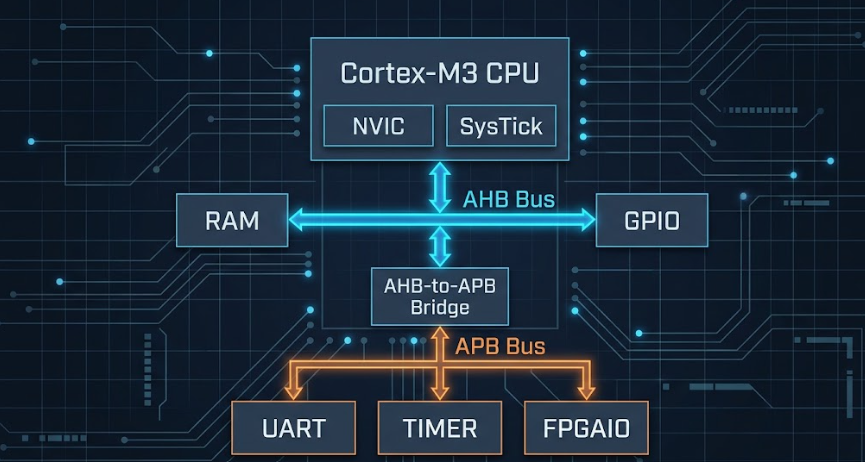
\includegraphics[width=0.5\textwidth]{contents/images/week_03/BUS_Panoramic.png}
    \caption{Panoramica funzionamento BUS}
\end{figure}

\subsection{La Topologia dei Bus: AHB e APB}
A livello hardware, il sistema non è piatto: i componenti sono distribuiti su reti diverse (chiamate \textit{Bus}) in base alla velocità e all'energia richiesta.

\begin{itemize}
    \item \textbf{Il Cuore della CPU (Core Peripherals):} Componenti vitali come il \textbf{SysTick} (il timer di sistema) e il \textbf{NVIC} (il gestore degli interrupt) sono integrati direttamente nel processore Cortex-M3. La CPU vi accede istantaneamente per gestire le emergenze, senza passare per reti esterne.
    \item \textbf{Bus ad Alta Velocità (Bus AHB):} L'\textit{Advanced High-performance Bus} è la rete principale del sistema, capace di scambiare dati alla massima velocità. Viene utilizzata per collegare la \textbf{RAM} (memoria) e il controller \textbf{GPIO}.
    \item \textbf{La Rete Secondaria (Bus APB):} L'\textit{Advanced Peripheral Bus} è una rete più lenta e a basso consumo energetico. Ospita i dispositivi esterni come la porta \textbf{UART} e i \textbf{Timer}. Per permettere alla CPU di parlare con questa rete, i dati viaggiano sul bus AHB e attraversano un traduttore hardware chiamato \textbf{AHB-to-APB Bridge}.
\end{itemize}

\subsection{Dalla Simulazione al Bare-Metal: Il Ruolo della UART0}
Nelle settimane precedenti, il nostro codice stampava messaggi a schermo usando il \textbf{semihosting}. Questa tecnica è di fatto una "scorciatoia": il processore si bloccava e chiedeva al computer esterno (tramite il debugger) di stampare il testo al posto suo.

Un vero sistema operativo \textit{bare-metal} (indipendente e a basso livello) deve però gestire l'hardware da solo. Per farlo, utilizziamo l'\textbf{UART} (\textit{Universal Asynchronous Receiver-Transmitter}), ovvero la porta seriale del microcontrollore, dotata di un canale di trasmissione (\textbf{TX}) e uno di ricezione (\textbf{RX}).

\textbf{Perché comunichiamo tramite la UART0?}\\
La scheda emulata possiede diverse porte seriali, ma noi utilizziamo l'\texttt{UART0} all'indirizzo \texttt{0x40004000} per un motivo pratico legato al nostro emulatore. Quando avviamo QEMU tramite il comando \texttt{make run}, utilizziamo il flag \texttt{-serial stdio}. 
Questo comando dice a QEMU di prendere i cavi virtuali TX e RX dell'\texttt{UART0} e collegarli direttamente alla nostra finestra del terminale. Di conseguenza:
\begin{itemize}
    \item Quando il nostro codice C scrive un byte (es. la lettera 'A') nel registro \texttt{DATA} dell'\texttt{UART0}, l'hardware lo invia sul cavo TX e QEMU lo stampa a schermo.
    \item Quando premiamo un tasto sulla tastiera, QEMU inietta quel carattere sul cavo RX, permettendo al nostro software di leggerlo interrogando lo stesso registro.
\end{itemize}

\section{The Dangers of Read-Modify-Write (RMW)}
When configuring a hardware device, we often need to change a single bit while leaving the rest of the register untouched. In C, it is natural to use compound operators like \texttt{|=} (e.g., \texttt{CMSDK\_GPIO0->DATAOUT |= (1u << 3)}). 

Even though this looks like a single, instant operation in your code, the processor is forced to execute three distinct steps at the hardware level:
\begin{enumerate}
    \item \textbf{Read:} It loads the current value of the register from memory into the CPU.
    \item \textbf{Modify:} It mathematically alters the target bit using a bitwise operation.
    \item \textbf{Write:} It saves the new value back, overwriting the hardware register.
\end{enumerate}

\begin{figure}[h]
    \centering
    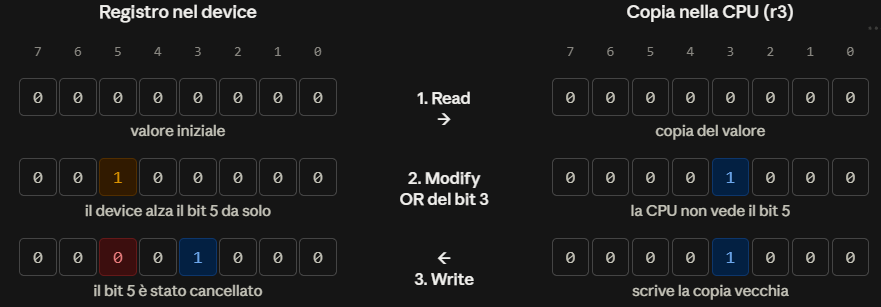
\includegraphics[width=0.5\textwidth]{contents/images/week_03/Read-Modify-Write.png}
    \caption{Read - Modify - Write}
\end{figure}

This sequence is \textbf{not atomic}, meaning it can be interrupted halfway through. This introduces three classic pitfalls when writing device drivers:

\begin{itemize}
    \item \textbf{Concurrency conflicts:} If an interrupt fires (or the hardware autonomously changes another bit) between your Read and Write phases, your final Write will forcefully overwrite the entire register with the outdated data you initially read, effectively erasing the hardware's recent changes.
    \item \textbf{The W1C (Write-1-to-Clear) Trap:} Many status registers turn off an alarm (flag) when you write a \texttt{1} to them. If you use an RMW pattern (\texttt{|=}) here, you will read back all the currently active alarms (as \texttt{1}s) and write them straight back, accidentally resetting every pending interrupt flag at once.
    \item \textbf{Read/Write Asymmetry:} In some registers, what you read means something entirely different from what you write. A Read-Modify-Write cycle on these registers will scramble the bits unpredictably.
\end{itemize}

\begin{figure}[h]
    \centering
    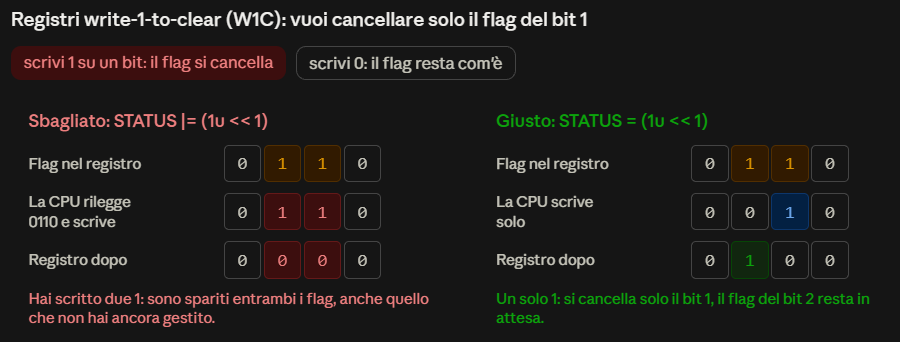
\includegraphics[width=0.5\textwidth]{contents/images/week_03/W1C.png}
    \caption{Write 1 to Clean Trap}
\end{figure}

\subsection{Safer Hardware Patterns}
To communicate with registers safely, adopt these practices:
\begin{itemize}
    \item \textbf{Use Dedicated Registers (Set/Clear):} Modern peripherals offer special registers (like \texttt{OUTENABLESET}) designed to be used with a simple direct assignment (\texttt{=}). The hardware handles it internally, ensuring only the bits set to \texttt{1} are modified in a single, safe operation.
    \item \textbf{How to Handle W1C:} To clear a flag in a W1C register, \textbf{always} use a direct assignment (\texttt{=}) targeting only the specific bit you want to clear. \textbf{Never} use \texttt{|=}.
    \item \textbf{Careful with C Bit-Shifts:} Always write \texttt{1u << n} rather than \texttt{1 << n}. The \texttt{u} forces the compiler to treat the number as unsigned. Shifting a signed \texttt{1} into the 31st bit is undefined behavior in C and will cause glitches.
\end{itemize}

\begin{figure}[h]
    \centering
    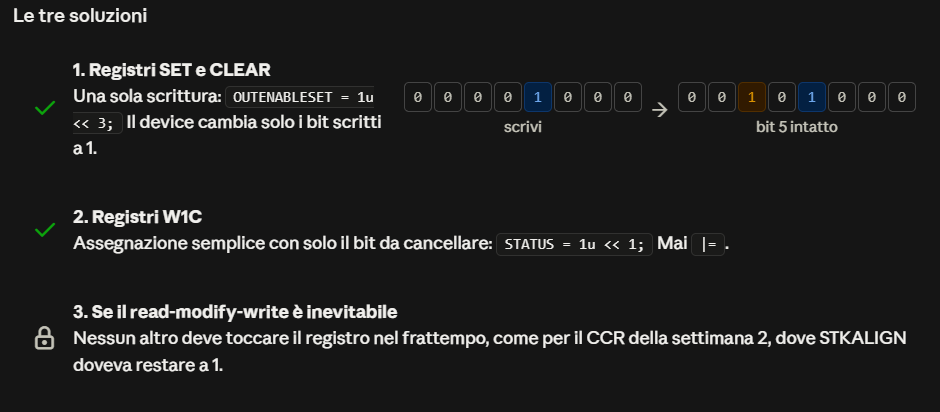
\includegraphics[width=0.5\textwidth]{contents/images/week_03/Read-Modify-Write Solutions.png}
    \caption{Read - Modify - Write Solutions}
\end{figure}

\section{The Device Protocol and the Driver Concept}

A \textbf{device driver} is a dedicated piece of software that acts as a translator between the operating system and the physical hardware. Instead of forcing the main application to memorize memory addresses and bitwise operations, the driver hides this complexity behind a clean API boundary. 

It offers the rest of the system \textbf{functions with a clear meaning} (e.g., \texttt{uart\_putc('A')} to "send this byte"), while internally dealing with the strict hardware rules. Callers simply include the driver's header (\texttt{drivers/uart.h}) and never touch the raw register map (\texttt{cmsdk.h}).

\subsection{The Hardware State Machine}
Interacting with a hardware device is never as simple as writing to a single variable. It requires following a strict state machine protocol dictated by the device's manual. A device is a \textbf{protocol} expressed through its registers, always executed in a fixed, logical sequence:

\begin{enumerate}
    \item \textbf{Configure} (e.g., \texttt{BAUDDIV}): Set up the operating parameters before turning anything on. For a UART, this means calculating and setting the transmission speed (baud rate).
    \item \textbf{Enable} (e.g., \texttt{CTRL}): Power on the specific sub-components (like the transmitter or receiver). You must enable the device \textit{only after} it has been fully configured.
    \item \textbf{Check Status} (e.g., \texttt{STATE}): Never blindly send or receive. You must read the status flags to ensure the hardware buffer actually has room to accept a new byte, or that a new incoming byte is truly waiting to be read.
    \item \textbf{Move Data} (e.g., \texttt{DATA}): Once the status is confirmed to be clear and ready, you can safely read or write the actual data payload.
    \item \textbf{Acknowledge} (e.g., \texttt{INTSTATUS}): If the device generated an event (such as triggering an interrupt), you must clear its specific flag to tell the hardware you have handled the event, allowing it to report the next one.
\end{enumerate}

\begin{figure}[h]
    \centering
    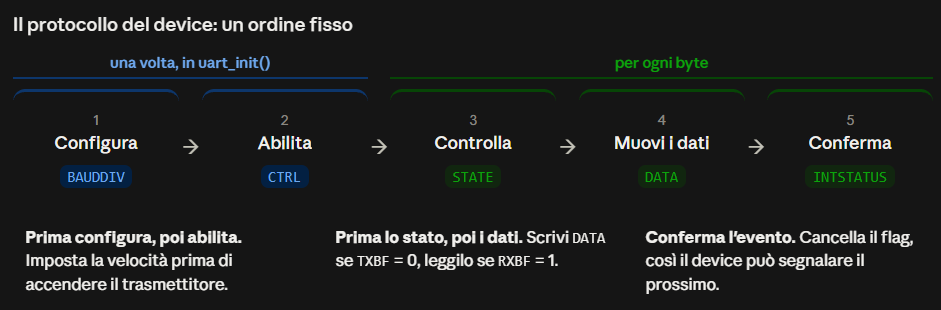
\includegraphics[width=0.5\textwidth]{contents/images/week_03/device_driver_protocol.png}
    \caption{Device Driver Protocol - steps}
\end{figure}

\subsubsection{Configuring the Baud Rate}
Because UART is asynchronous, both devices must agree on a transmission speed (baud rate). You divide your CPU's clock frequency by your target baud rate. If our CPU runs at 25 MHz and we want 115,200 baud:
\[ \text{BAUDDIV} = \frac{25,000,000}{115,200} \approx 217 \]
Writing 217 into \texttt{BAUDDIV} configures the hardware correctly.

\begin{figure}[h]
    \centering
    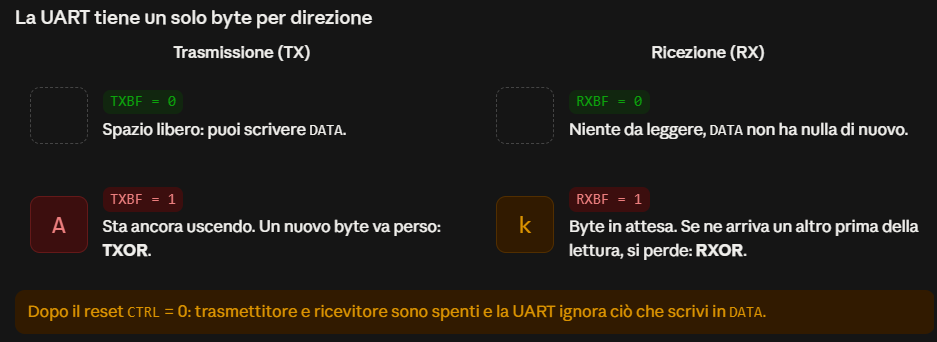
\includegraphics[width=0.5\textwidth]{contents/images/week_03/TX-RX.png}
    \caption{How transmission flags works}
\end{figure}

\section{Implementing the Device Driver}

\subsection{How Bigger OSes Generalize a Driver}
If a system has many character devices, the OS needs a generic way to talk to them. Operating systems solve this by defining a \texttt{struct} composed of function pointers:

\begin{lstlisting}
struct char_driver 
{
    void (*init)(void);          /* bring the device up */
    int  (*read)(void);          /* read one byte, or -1 if none */
    void (*write)(char c);       /* send one byte */
};

static const struct char_driver uart0_driver = { 
    uart_init, 
    uart_getc_polled, 
    uart_putc_polled 
};
\end{lstlisting}

This allows generic code to interact with any device (e.g., \texttt{dev->write('h');}) without knowing its specifics. Linux does exactly this with \texttt{struct file\_operations}. This week's kernel has a single console and calls the UART functions directly, so you will not write this \texttt{struct} yet.

\subsection{Implementing and Using the UART Driver}
In \texttt{drivers/uart.c}, paste the following right \textbf{above} the marker line \texttt{/* CLASS: uart\_init, polled putc/getc, ...} (keep the marker for Unit~2).

\begin{lstlisting}
#include "drivers/uart.h"
#include "cmsdk.h"

void uart_init(void)
{
    /* configure: speed (QEMU ignores it) */
    CMSDK_UART0->BAUDDIV = 16;
    /* enable: transmitter and receiver */
    CMSDK_UART0->CTRL = UART_CTRL_TXEN | UART_CTRL_RXEN;
}

void uart_putc_polled(char c)
{
    /* check status: wait for room */
    while (CMSDK_UART0->STATE & UART_STATE_TXBF)
    {
    }
    /* move data: send the byte */
    CMSDK_UART0->DATA = (uint32_t)(unsigned char)c;
}
\end{lstlisting}

Following the protocol, \texttt{uart\_init} configures and enables the hardware. Because the UART is an external physical device, initialization happens only \textbf{once} at boot. We combine two bitmasks with a bitwise OR to enable both directions simultaneously. 

In \texttt{uart\_putc\_polled}, if the \texttt{TXBF} bit is 1, the CPU loops waiting; once free, the byte is stored into \texttt{DATA}. 
\textbf{Why the double cast?} On Arm, \texttt{char} is unsigned, but on many compilers it is signed. A signed \texttt{char} holding \texttt{0xE9} is $-23$, which converts to \texttt{uint32\_t} as \texttt{0xFFFFFFE9}. Casting through \texttt{unsigned char} ensures it becomes \texttt{0x000000E9}, extracting exactly the byte.

\paragraph{Testing the Driver}
In \texttt{src/main.c}, add \texttt{\#include "drivers/uart.h"} above \texttt{main}, and right after the marker \texttt{/* CLASS: bring up the UART here */} add:

\begin{lstlisting}
#include "drivers/uart.h"

int main(void)
{
    /* CLASS: bring up the UART here */
    uart_init();
    uart_putc_polled('O');
    uart_putc_polled('K');
    uart_putc_polled('\n');
    for (;;) { }
}
\end{lstlisting}

\texttt{make run} prints \texttt{OK}: the first real hardware output of our OS. 
If you comment out \texttt{uart\_init()}, \texttt{CTRL} remains 0 and the UART drops every byte. Running QEMU with \texttt{-d guest\_errors} reports:
\begin{lstlisting}[language=bash]
CMSDK APB UART: transmit data write with Tx disabled
\end{lstlisting}
This enforces the rule ``enable before moving data''.

\subsection{Try It: A Polled Echo}
In \texttt{drivers/uart.c}, right after \texttt{uart\_putc\_polled}, add the reading function. It returns \texttt{-1} immediately if no character is waiting:

\begin{lstlisting}
int uart_getc_polled(void)
{
    /* check status: nothing received yet */
    if ((CMSDK_UART0->STATE & UART_STATE_RXBF) == 0)
    {
        return -1;
    }
    /* move data: reading DATA takes the byte */
    return (int)(CMSDK_UART0->DATA & 0xFF);
}
\end{lstlisting}

In \texttt{src/main.c}, replace the empty \texttt{for (;;) \{ \}} at the end of \texttt{main} with an echo loop:

\begin{lstlisting}
    for (;;)
    {
        int c = uart_getc_polled();
        if (c >= 0)            /* -1: no key */
        {
            uart_putc_polled((char)c);
        }
    }
\end{lstlisting}

Run \texttt{make run} and type \texttt{hello}. With \texttt{-nographic}, the terminal does not show what you type: every letter you see was \textbf{sent back by your program}. The Enter key sends a carriage return (\texttt{\textbackslash r}), jumping the cursor back to the start of the line. The CPU spins in this loop millions of times per second: this is the price of polling.

\section{Variadic Functions and \texttt{<stdarg.h>}}
Currently, our driver can only print single characters. To build a true operating system, we need a \texttt{printf}-like function capable of formatting complex strings and numbers (e.g., \texttt{\%d}, \texttt{\%s}, \texttt{\%x}). We will call our kernel-level version \texttt{kprintf}.

To build \texttt{kprintf}, we face two tasks:
\begin{enumerate}
    \item String formatting (parsing the \texttt{\%d} markers and converting integers to ASCII characters).
    \item Sending the resulting characters to the UART.
\end{enumerate}

In C, a function that accepts an arbitrary number of arguments (like \texttt{printf}) is called a \textbf{variadic function}. It is declared using an ellipsis (\texttt{...}):

\begin{lstlisting}
void kprintf(const char *fmt, ...);
\end{lstlisting}

\texttt{<stdarg.h>} is one of the headers a freestanding build still gives you, as you saw in Week~2: it contains only types and compiler built-ins, no library code. Behind the scenes, it provides macros to navigate the memory (the stack or registers) where the extra arguments are stored. Here is exactly what the macros do:

\begin{itemize}
    \item \textbf{\texttt{va\_list ap}:} Think of this as an ``argument pointer'' (hence \texttt{ap}). It is a special cursor variable that keeps track of your current position within the hidden list of extra arguments.
    \item \textbf{\texttt{va\_start(ap, fmt)}:} This initializes the cursor. By passing the last known fixed argument (\texttt{fmt}), the compiler calculates exactly where in memory the variable arguments begin.
    \item \textbf{\texttt{va\_arg(ap, int)}:} This macro performs two actions simultaneously. First, it reads the value at the cursor's current position (interpreting it as the specified type, like \texttt{int}). Second, it automatically advances the cursor by the exact number of bytes required to reach the next argument.
    \item \textbf{\texttt{va\_end(ap)}:} This cleans up the cursor. While on some architectures (like our Cortex-M3) it might do nothing behind the scenes, it is strictly mandatory for C standard compliance and prevents memory corruption on more complex systems.
\end{itemize}

\begin{lstlisting}
#include <stdarg.h>

void kprintf(const char *fmt, ...)
{
    va_list ap;                  /* 1. create the cursor */
    va_start(ap, fmt);           /* 2. point it right after 'fmt' */
    int n = va_arg(ap, int);     /* 3. read the first extra arg as int, advance cursor */
    va_end(ap);                  /* 4. clean up */
}
\end{lstlisting}

A variadic function cannot see how many arguments it received, nor their types.
The \textbf{format string} tells it: \texttt{\%d} means ``take an \texttt{int}''.
If the type in the format and the type actually passed disagree, the behavior is
undefined. Arguments passed through \texttt{...} are also \textbf{promoted}: a
\texttt{char} arrives as an \texttt{int}, so \texttt{\%c} must read it with
\texttt{va\_arg(ap, int)}.

By convention, a function that receives a \texttt{va\_list} instead of \texttt{...} has a name starting with \texttt{v}, such as \texttt{vprintf} in the C library. The \emph{C for device drivers} tutorial (Section~4) shows variadic functions, promotions and a tiny format dispatcher you can run on your laptop.

\subsection{Separating Formatting from Output (\texttt{vformat})}
Turning \texttt{"x=\%d"} and \texttt{42} into \texttt{x=42} is the same work wherever the characters end up. So \texttt{lib/format.h} (given) separates \textbf{what} to print from \textbf{where} it goes:

To maintain a clean operating system architecture, we separate the formatting engine from the hardware driver using a function called \texttt{vformat} (implemented in \texttt{lib/format.c}). 

\begin{lstlisting}
void vformat(void (*out)(char c, void *ctx), void *ctx,
             const char *fmt, va_list ap);
\end{lstlisting}

The \texttt{out} parameter is a \textbf{function pointer}. Instead of hardcoding \texttt{uart\_putc\_polled} directly inside the formatting loop, we pass the output function as a variable. \texttt{vformat} calls \texttt{out(c, ctx)} once for every character it produces. This decouples the logic: \texttt{vformat} formats text, completely unaware of whether the characters are going to a UART, a screen, or a network socket.

The \texttt{void *ctx} (context) is an \textbf{opaque pointer}. This is a standard C design pattern used to pass arbitrary state data through a generic function. \texttt{vformat} does not know or care what \texttt{ctx} points to; it simply receives it and hands it untouched to your \texttt{out} function. If your output function needs to keep track of a string buffer or a character counter, you pass a pointer to that structure as \texttt{ctx}. 

\texttt{kprintf} is then built by calling \texttt{vformat} with an \texttt{out} function that calls \texttt{uart\_putc\_polled}. Since a UART just blasts characters out and requires no memory state tracking, we simply pass \texttt{0} (or \texttt{NULL}) as the \texttt{ctx}. 

Another destination needs only another small \texttt{out} function: the formatting is written and tested once.

\texttt{vformat} supports \texttt{\%c}, \texttt{\%s}, \texttt{\%d} (signed decimal), \texttt{\%u} (unsigned decimal), \texttt{\%x} (hexadecimal, lowercase, without \texttt{0x}) and \texttt{\%\%} (a percent sign). 

There is no width and no precision, and an unknown conversion such as \texttt{\%q} is printed as written.

The two helpers that turn a number into text, \texttt{utoa\_dec} and \texttt{utoa\_hex}, are already in \texttt{lib/format.c} in the base.

\subsection{Writing \texttt{vformat}}
In \texttt{lib/format.c}, replace the marker line \texttt{/* CLASS: vformat (the \% dispatch: \%c \%s \%d \%u \%x \%\%) goes here. */} with a helper and the function itself. 

The helper, \texttt{put\_string}, sends every character of a string to \texttt{out}:

\begin{lstlisting}
static void put_string(void (*out)(char c, void *ctx), void *ctx,
                       const char *s)
{
    while (*s != '\0')
    {
        out(*s, ctx);
        s++;
    }
}
\end{lstlisting}

\texttt{vformat} walks through the format string. An ordinary character is passed on; a \texttt{\%} makes it look at the next letter and take one argument of the right type:

\begin{lstlisting}
void vformat(void (*out)(char c, void *ctx), void *ctx,
             const char *fmt, va_list ap)
{
    char num[12];   /* longest number + '\0' */

    while (*fmt != '\0')
    {
        if (*fmt != '%')                /* ordinary character: pass it on */
        {
            out(*fmt, ctx);
            fmt++;
            continue;
        }
        fmt++;                          /* a '%': look at the next letter */
        switch (*fmt)
        {
        case 'c':
            out((char)va_arg(ap, int), ctx);   /* a char arrives as an int */
            break;
        case 's':
        {
            const char *s = va_arg(ap, const char *);
            put_string(out, ctx, s != 0 ? s : "(null)");  /* no crash on null */
            break;
        }
        case 'd':
        {
            int v = va_arg(ap, int);
            uint32_t mag;
            if (v < 0) { out('-', ctx); mag = 0u - (uint32_t)v; }
            else       { mag = (uint32_t)v; }
            utoa_dec(mag, num);
            put_string(out, ctx, num);
            break;
        }
        case 'u': utoa_dec(va_arg(ap, uint32_t), num); put_string(out, ctx, num); break;
        case 'x': utoa_hex(va_arg(ap, uint32_t), num); put_string(out, ctx, num); break;
        case '%': out('%', ctx); break;
        case '\0': out('%', ctx); return;                  /* string ended after '%' */
        default:  out('%', ctx); out(*fmt, ctx); break;    /* unknown: as written */
        }
        fmt++;                          /* past the conversion letter */
    }
}
\end{lstlisting}

(The solution file spreads the same code over more lines, with a comment on each.)

\paragraph{Why \texttt{0u - (uint32\_t) v} and not \texttt{-v}?} 
Because the most negative \texttt{int}, $-2\,147\,483\,648$ (\texttt{INT\_MIN}), has no positive \texttt{int} counterpart, so \texttt{-v} overflows, which is undefined behavior in C. 

Unsigned subtraction is always well defined, and gives $2\,147\,483\,648$. After this step \texttt{make} must build with no errors.

\section{The Kernel Print Function (\texttt{kprintf})}
With the formatting engine and the UART driver both ready, we can combine them to create a real print function. We name it \textbf{\texttt{kprintf}} (where the "k" stands for kernel). 

\subsection{Kernel Mode vs. User Mode Printing}
Naming this function \texttt{kprintf} highlights a fundamental operating system concept. In a real OS (like Linux), there is a strict separation between how the kernel prints messages and how a user application prints messages:

\begin{itemize}
    \item \textbf{User-Level \texttt{printf}:} A user application runs in a restricted user mode. It does not know that a UART even exists, nor does it have the hardware privileges to touch it. When a user program calls \texttt{printf}, it triggers a \texttt{system call}, asking the OS to print on its behalf. The OS then securely routes that request to the appropriate device driver.
    \item \textbf{Kernel-Level \texttt{kprintf}:} The OS kernel itself runs in privileged (supervisor) mode. It inherently knows about the hardware and the I/O devices. Therefore, \texttt{kprintf} bypasses system calls entirely and talks directly to the hardware driver. This is not only a design choice: the kernel \emph{cannot} use \texttt{printf} for its own messages, because an \texttt{svc} issued from the SVCall handler escalates to a HardFault.
\end{itemize}

Any operating system that implements hardware protection features both a user-side print function and a kernel-side print function. We are currently inside the operating system layer, so we implement \texttt{kprintf} first. (The more complex user-level system call mechanism will be implemented later).

\subsection{Implementing \texttt{kprintf}}
In \texttt{kernel/kprintf.c}, we write a small wrapper function that connects \texttt{vformat} to our polled UART driver.

First, we define the callback function that \texttt{vformat} expects. This simply takes a character and hands it to the hardware driver:
\begin{lstlisting}
#include "kernel/kprintf.h"
#include "lib/format.h"
#include "drivers/uart.h"

/* vformat's output: one char to the UART */
static void kprintf_out( char c, void *ctx ){
    (void) ctx;     /* tell the compiler this argument is intentionally unused */
    uart_putc_polled( c );
}
\end{lstlisting}

\paragraph{Why \texttt{(void) ctx}?} 
The \texttt{vformat} engine expects its output function to accept two arguments: the character to print and the context pointer (\texttt{ctx}). Our \texttt{kprintf\_out} function must accept both to match the required signature, even though a simple polled UART driver does not need any context state. Writing \texttt{(void) ctx;} is a standard C idiom: it explicitly tells the compiler that the parameter is intentionally ignored, suppressing the 'unused parameter' warning during compilation.

Then, we implement the variadic \texttt{kprintf} function itself. It collects its extra arguments into a \texttt{va\_list} and hands everything over to \texttt{vformat}, setting \texttt{kprintf\_out} as the destination and \texttt{0} (NULL) as the context:
\begin{lstlisting}
void kprintf( const char *fmt, ... )
{
    va_list ap;
    va_start( ap, fmt );
    vformat( kprintf_out, 0, fmt, ap );
    va_end( ap );
}
\end{lstlisting}

\paragraph{How the \texttt{va\_list} is passed:}
Notice that \texttt{kprintf} itself does not call \texttt{va\_arg} to read the arguments. It simply initializes the cursor (\texttt{ap}) with \texttt{va\_start}, and passes the whole cursor by value to \texttt{vformat}. It is the job of the \texttt{switch} statement inside \texttt{vformat} to call \texttt{va\_arg} and advance the cursor as it parses the format string. When \texttt{vformat} returns, \texttt{kprintf} cleans up the cursor with \texttt{va\_end}.

Because \texttt{kprintf} relies on our polled UART driver, it operates entirely without hardware interrupts. This is a massive architectural advantage: it means \texttt{kprintf} can be safely executed anywhere in the kernel, even inside a catastrophic \texttt{HardFault} handler where interrupts are strictly disabled.

To test every conversion, we can add a test line in \texttt{src/main.c}:
\begin{lstlisting}
kprintf( "c=%c s=%s d=%d u=%u x=%x pct=%%\n", 
                'A', "hi", -42, 4000000000u, 0xBEEFu );
\end{lstlisting}
This outputs \texttt{c=A s=hi d=-42 u=4000000000 x=beef pct=\%}. Notice that \texttt{\%x} prints no \texttt{0x} prefix; if you want one, you must write it explicitly in the format string (e.g., \texttt{"0x\%x"}).

You can follow a call by hand to check the \texttt{vformat} logic. For \texttt{kprintf("d=\%d\textbackslash{}n", -42)}:
\begin{itemize}
    \item The loop passes \texttt{d} and \texttt{=} to \texttt{kprintf\_out}.
    \item It meets \texttt{\%}, moves to \texttt{d}, takes an \texttt{int} (-42) with \texttt{va\_arg}.
    \item It sends \texttt{-}, computes the magnitude 42, turns it into the text \texttt{"42"} with \texttt{utoa\_dec}, and sends \texttt{4} and \texttt{2}.
    \item It moves past the \texttt{d}, passes \texttt{\textbackslash{}n}, and stops at the terminating zero.
\end{itemize}
This results in exactly six calls to \texttt{kprintf\_out}, pushing six bytes sequentially to the UART.

\section{Upgrading the Kernel: Fault Handlers That Print}
The base's fault handlers are silent infinite loops: if a hardware fault happens, the program simply stops answering. Now that the kernel can print using our robust, polled \texttt{kprintf}, the handlers can explicitly state what happened.

\subsection{The Status Registers (HFSR and CFSR)}
Two specific registers of the System Control Block (SCB) tell you why a fault happened:
\begin{itemize}
    \item \textbf{CFSR (Configurable Fault Status Register):} Located at \texttt{0xE000ED28}, this register has one specific bit for each possible cause of a \texttt{MemManage} fault, a \texttt{BusFault}, or a \texttt{UsageFault}.
    \item \textbf{HFSR (HardFault Status Register):} Located at \texttt{0xE000ED2C}, this indicates exactly why a \texttt{HardFault} was escalated. For example, bit~30 (\texttt{FORCED}, \texttt{0x40000000}) means that a fault was
escalated to HardFault.
\end{itemize}



\subsection{Implementing the New Handlers}
In \texttt{kernel/faults.c}, we include the necessary headers and replace the silent loops with explicit print statements before halting:
\begin{lstlisting}
#include "cmsdk.h"
#include "kernel/kprintf.h"

void HardFault_Handler(void) {
    kprintf( "HardFault: HFSR=0x%x\n", SCB->HFSR );
    for(;;){}
}
void MemManage_Handler(void) {
    kprintf( "MemManage: CFSR=0x%x\n", SCB->CFSR );
    for(;;){}
}
void BusFault_Handler(void) {
    kprintf( "BusFault: CFSR=0x%x\n", SCB->CFSR );
    for(;;){}
}
void UsageFault_Handler(void) {
    kprintf( "UsageFault: CFSR=0x%x\n", SCB->CFSR );
    for(;;){}
}
\end{lstlisting}

\subsection{Try It: Catching a Divide-By-Zero}
To test this new capability, we can intentionally crash the OS. Week 2's \texttt{Reset\_Handler} set the \texttt{DIV\_0\_TRP} bit in the CCR, meaning an integer division by zero strictly triggers a hardware fault. 

Add the following temporary code to \texttt{src/main.c}:
\begin{lstlisting}
volatile unsigned zero = 0;     /* read at run time */
kprintf( "%u\n", 10u / zero );  /* should fault     */
\end{lstlisting}
The \texttt{volatile} keyword is crucial here; it forces the compiler to perform the math at runtime rather than computing the result at build time.

Running \texttt{make run} yields:
\begin{verbatim}
UsageFault: CFSR=0x2000000
\end{verbatim}

The value \texttt{0x2000000} indicates that bit 25 is set, which perfectly corresponds to \texttt{SCB\_CFSR\_DIVBYZERO} in \texttt{include/cmsdk.h}. The CPU instantly fired a \texttt{UsageFault}, the handler used the polled \texttt{kprintf} to push the error string over the UART, and then the system cleanly locked up in the infinite loop.

\subsection{Practical Note: Project Navigation and Exam Expectations}
As we build these low-level layers, the codebase is becoming increasingly complex. Files are spread across different directories (\texttt{drivers/}, \texttt{kernel/}, \texttt{lib/}, \texttt{src/}), each serving a distinct architectural role.

From an academic and practical standpoint, it is critical to understand how to navigate this project structure. During an exam (or in a real-world debugging scenario), you will not be asked to write a full operating system from scratch in 90 minutes. Instead, you will typically be given an existing, structured project and asked to implement a specific function, fix a bug, or integrate a new hardware feature. Mastering how to read the existing code, locate the correct files, and understand the flow of execution is just as important as understanding the hardware registers themselves.


\section{Unit 2: Calling Convention and Interrupts}
Up to this point, our entire OS relies on \textbf{polling}. The \texttt{uart\_putc\_polled} driver explicitly reads the hardware \texttt{STATE} register in an infinite loop until the transmitter has room.

\subsection{Polling versus Interrupts}
While polling is easy to implement, it is unsustainable for a real operating system. The alternative is an \textbf{interrupt}: the hardware device sends a physical signal only when it actually needs attention. The CPU pauses instantly, runs a special function called a \textit{handler}, and then resumes exactly where it left off.

\begin{table}[h!]
    \centering
    \begin{tabular}{p{2.5cm}p{5.5cm}p{6cm}}
        \toprule
        & \textbf{Polling} & \textbf{Interrupts} \\
        \midrule
        \textbf{CPU Time} & Wasted in an empty waiting loop. & Used only when the event actually occurs. \\
        \textbf{Latency} & Up to one full loop iteration. & The exception entry time ($\sim$12 cycles on Cortex-M3). \\
        \textbf{Complexity} & Trivial; a single loop. & Complex: requires handlers, data protection, and priority management. \\
        \textbf{CPU State} & Constantly locked at 100\% usage. & Free to run applications or enter sleep mode. \\
        \bottomrule
    \end{tabular}
\end{table}

To understand the real cost of polling: sending 10 bits at 115,200 baud takes about 87~$\mu$s. At our board's 25~MHz clock, that equals \textbf{2,170 clock cycles}. With polling, the CPU wastes all these cycles just spinning and doing nothing. 

However, polling remains vital when interrupts cannot work. This is why our \texttt{kprintf} will stay polled: it must guarantee output even when the system crashes inside a \texttt{HardFault} (where normal interrupts are strictly blocked).

\subsection{The AAPCS: How C Calls Functions}
To make C and Assembly code work together, both must follow strict rules on how to exchange data. For the ARM architecture, this standard is the \textbf{AAPCS} (Procedure Call Standard for the Arm Architecture).

The standard assigns precise roles to the CPU registers:
\begin{itemize}
    \item \textbf{\texttt{r0--r3}:} Carry the first four parameters of a function. The \texttt{r0} register also holds the final return value. These are \textbf{Caller-Saved} (scratch) registers: the called function can overwrite them freely without asking for permission.
    \item \textbf{\texttt{r4--r11}:} Reserved for the function's local variables. These are \textbf{Callee-Saved}: if a function uses them, it is strictly required to back them up (via \texttt{push}) and restore them (\texttt{pop}) before returning.
    \item \textbf{\texttt{r12}:} A temporary scratch register, strictly \textbf{Caller-Saved}.
    \item \textbf{\texttt{lr} (Link Register):} Holds the address the CPU must return to when the function ends. Since it is \textbf{Caller-Saved}, if a function calls another function, it must save its own \texttt{lr} first.
    \item \textbf{\texttt{sp} (Stack Pointer):} The stack memory address must always remain a multiple of 8 at every function boundary.
\end{itemize}

\subsection{Managing Interrupts from Assembly: The PRIMASK}
Before handling specific hardware interrupts, the OS needs a main switch to globally enable or disable the CPU's ability to listen. The Cortex-M3 has a special 1-bit register called \textbf{PRIMASK}. When \texttt{PRIMASK} is \texttt{1}, all configurable interrupts are masked (blocked); when \texttt{0}, the CPU is listening.

Standard C cannot touch the CPU's internal registers. We must use specific Assembly instructions:
\begin{itemize}
    \item \texttt{mrs r0, primask}: Reads the value of \texttt{PRIMASK} and saves it into \texttt{r0}.
    \item \texttt{msr primask, r0}: Writes the content of \texttt{r0} into \texttt{PRIMASK}.
    \item \texttt{cpsid i} / \texttt{cpsie i}: Quick instructions to disable (\textit{disable}) or enable (\textit{enable}) global interrupts.
\end{itemize}

\subsubsection{The Nesting Problem}
A naive approach to protecting a critical section of code is to use \texttt{cpsid i} at the start and \texttt{cpsie i} at the end. However, if a function that disables interrupts calls another function that does the same, the inner function will turn the interrupts back on when it finishes, destroying the protection of the outer function way too early.

The correct solution requires functions to save the previous state before changing it:
\begin{lstlisting}
uint32_t irq_save( void );         /* Blocks interrupts and returns the old PRIMASK */
void irq_restore( uint32_t old );  /* Restores PRIMASK to the saved state */
\end{lstlisting}
This way, even with nested calls, interrupts will only be truly re-enabled when the outermost function restores the original \texttt{0} value.

\subsubsection{Implementing \texttt{irq\_save} and \texttt{irq\_restore} in Assembly}
We create these two functions in \texttt{kernel/irq.s}. Following the AAPCS, \texttt{irq\_save} must place the old value into the \texttt{r0} register before returning to C. Both functions only use \texttt{r0} and \texttt{lr} (which are Caller-Saved), so we do not need to use \texttt{push} or \texttt{pop}.

\begin{lstlisting}
    .syntax unified             /* Modern ARM syntax */
    .cpu cortex-m3              /* Limit to our chip's instructions */
    .thumb                      /* Use the Thumb instruction set */
    .section .text,"ax",%progbits

/* uint32_t irq_save(void) */
    .global irq_save            /* Make the name visible to the C linker */
    .type irq_save, %function   /* Declare this as executable code */
    .thumb_func                 
irq_save:
    mrs r0, primask             /* Save the old PRIMASK in r0 (return value) */
    cpsid i                     /* Set PRIMASK to 1 (mask interrupts) */
    bx lr                       /* Return to C */
    .size irq_save, . - irq_save

/* void irq_restore(uint32_t old) */
    .global irq_restore         
    .type irq_restore, %function 
    .thumb_func                 
irq_restore:
    msr primask, r0             /* Restore PRIMASK by reading it from r0 (the parameter) */
    bx lr                       /* Return to C */
    .size irq_restore, . - irq_restore
\end{lstlisting}

\subsubsection{Testing the API in C}
Let's define the prototypes in \texttt{kernel/irq.h}:

\begin{lstlisting}
#ifndef IRQ_H
#define IRQ_H
#include <stdint.h>

uint32_t irq_save(void);
void irq_restore(uint32_t state);

#endif
\end{lstlisting}

And test them inside \texttt{src/main.c}:

\begin{lstlisting}
#include "kernel/irq.h"

/* Inside main() */
uint32_t old_state = irq_save();      /* Save current state and block interrupts */

/* --- CRITICAL SECTION START ---
   In here, interrupts are safely blocked.
   ------------------------------ */

irq_restore(old_state);               /* Restore the previous state */

kprintf("PRIMASK before irq_save was: %u\n", old_state);
\end{lstlisting}

Execution will print \texttt{0}. This confirms the CPU started with interrupts enabled, our assembly safely disabled and cleanly restored them, communicating perfectly with the C code.

\subsubsection{Inspecting the AAPCS with GDB}
You can watch live how data travels between C and Assembly using GDB:
\begin{lstlisting}[language=bash]
(gdb) break irq_save
(gdb) continue
(gdb) p/x $lr
(gdb) info registers primask
(gdb) finish
(gdb) info registers r0 primask
\end{lstlisting}

At the breakpoint, the \texttt{lr} (Link Register) contains the return address generated by C, and \texttt{PRIMASK} is \texttt{0}. The \texttt{finish} command runs the assembly function to completion. By checking the registers again, you will see that \texttt{r0} now contains the old state (\texttt{0x0}) and \texttt{PRIMASK} has flipped to \texttt{1} (interrupts disabled). Everything moved exactly as dictated by the AAPCS rules.

\section{ARM Exception Entry and Return Mechanics}
While we can wrap many features in simple C functions, handling exceptions requires a deep understanding of what the Cortex-M hardware does autonomously. When a hardware interrupt fires, the CPU abruptly pauses the current execution to jump to an Exception Handler. Before executing the handler's first instruction, the hardware performs three critical operations:
\begin{enumerate}
    \item It pushes exactly 8 words (the exception frame) onto the current stack.
    \item It writes a special signature value, called \texttt{EXC\_RETURN}, into the Link Register (\texttt{lr}).
    \item It reads the specific handler's memory address from the vector table and branches to it, automatically elevating to privileged Handler mode.
\end{enumerate}

\subsection{The Automatic Hardware State Save (Stacking)}
The 8 words pushed to the stack form the stacked frame. Because the stack grows downwards, the hardware creates the following memory layout relative to the new Stack Pointer (\texttt{sp}):
\begin{itemize}
    \item \texttt{sp + 28}: \texttt{xPSR} (Status flags, Thumb bit)
    \item \texttt{sp + 24}: \texttt{PC} (Program Counter: where the interrupted code will resume)
    \item \texttt{sp + 20}: \texttt{LR} (The interrupted code's Link Register)
    \item \texttt{sp + 16}: \texttt{r12}
    \item \texttt{sp + 12}: \texttt{r3}
    \item \texttt{sp +  8}: \texttt{r2}
    \item \texttt{sp +  4}: \texttt{r1}
    \item \texttt{sp +  0}: \texttt{r0} $\leftarrow$ \texttt{sp} when the handler starts
\end{itemize}

Crucially, these registers (\texttt{r0}--\texttt{r3}, \texttt{r12}, and \texttt{lr}) perfectly match the AAPCS \textit{Caller-Saved} set. Because \texttt{r4}--\texttt{r11} are \textit{Callee-Saved}, any standard C function invoked during the interrupt will safely preserve them before modifying them. Together, the hardware stacking and the AAPCS software rules guarantee that the interrupted application finds all its registers entirely unmodified upon return. This elegant design allows an interrupt handler to be written as a standard C function (e.g., \texttt{void SysTick\_Handler(void)}) without requiring specialized assembly wrappers or keywords. Additionally, the hardware ensures the stack pointer remains 8-byte aligned upon entry, adhering to the \texttt{STKALIGN} bit configured in the CCR during boot.

\subsection{Exception Return: \texttt{EXC\_RETURN}}
Inside the exception handler, the \texttt{lr} does not contain a standard return memory address. Instead, it holds the \texttt{EXC\_RETURN} value, which begins with \texttt{0xFFFFFF...}---an address region deliberately containing no executable code. When the handler concludes and executes a return instruction (like \texttt{bx lr} or \texttt{pop \{..., pc\}}), the CPU hardware intercepts this special value and initiates an \textbf{exception return}. It pops the 8-word frame from the stack, reverts to the previous execution mode, and seamlessly resumes at the stacked \texttt{PC}.

\begin{table}[h!]
    \centering
    \begin{tabular}{lll}
        \toprule
        \textbf{\texttt{EXC\_RETURN}} & \textbf{Return To} & \textbf{Stack Used} \\
        \midrule
        \texttt{0xFFFFFFF9} & Thread mode (normal code, e.g., \texttt{main}) & Main stack \\
        \texttt{0xFFFFFFF1} & Handler mode (returning to a preempted handler) & Main stack \\
        \texttt{0xFFFFFFFD} & Thread mode & Process stack \\
        \bottomrule
    \end{tabular}
\end{table}

While the Cortex-M supports a secondary Process Stack Pointer, this kernel exclusively uses the Main stack for now. Therefore, returning to Thread mode will consistently utilize \texttt{0xFFFFFFF9}. The compiled C handler ends with an ordinary \texttt{bx lr}; the magic lies entirely in the value held within the Link Register.

\subsection{Tail-Chaining and Late Arrival}
To optimize back-to-back exceptions, the hardware utilizes two advanced mechanisms that require no software intervention:
\begin{itemize}
    \item \textbf{Tail-chaining:} If a handler completes while another exception is pending, the CPU skips the redundant process of popping the 8-word frame only to immediately push it again. Instead, it branches directly to the pending handler, reducing latency to about 6 cycles (down from 24) on a Cortex-M3.
    \item \textbf{Late arrival:} If a higher-priority exception arrives while the CPU is actively stacking the frame for a lower-priority exception, the CPU simply uses the partially completed frame, executes the higher-priority handler first, and then tail-chains to the lower-priority one.
\end{itemize}
In both scenarios, the single stacked frame explicitly describes the original code that was preempted.

\section{The Heartbeat of the OS: The SysTick Timer}
To build an operating system capable of measuring time and preempting tasks, a periodic interrupt is mandatory. The \textbf{SysTick} timer is a 24-bit down-counter permanently integrated into every Cortex-M core, mapped to the exact same memory addresses across all chips.

\subsection{Hardware Preemption}
If an OS relies entirely on cooperative software, an infinite loop in a user program would permanently hijack the CPU, deadlocking the system. SysTick prevents this through \textbf{hardware preemption}. By periodically firing an interrupt (e.g., every 10~ms), the hardware forcefully pauses the current execution and jumps to the kernel's \texttt{SysTick\_Handler}. This guarantees the OS regains control at fixed intervals to update the system clock, perform scheduling, or terminate rogue tasks. A hardware interrupt is the only mechanism powerful enough to definitively stop the CPU.

\subsection{The SysTick Hardware Registers}
The timer operates by counting down from a configured \texttt{LOAD} value to 0, reloading the \texttt{LOAD} value on the subsequent clock cycle. Consequently, exactly one period equals $\text{LOAD} + 1$ cycles.

\begin{table}[h!]
    \centering
    \begin{tabular}{llp{9cm}}
        \toprule
        \textbf{Register} & \textbf{Address} & \textbf{Function} \\
        \midrule
        \textbf{\texttt{CTRL}} & \texttt{0xE000E010} & Bit 0: \textbf{ENABLE} the counter. Bit 1: \textbf{TICKINT} (raise the SysTick exception at 0). Bit 2: \textbf{CLKSOURCE} (1 = processor clock). Bit 16: \textbf{COUNTFLAG} (reads 1 if 0 was reached since last read). \\
        \textbf{\texttt{LOAD}} & \texttt{0xE000E014} & 24-bit reload value (maximum \texttt{0xFFFFFF}). \\
        \textbf{\texttt{VAL}} & \texttt{0xE000E018} & Current count. Writing any value resets it to 0. \\
        \textbf{\texttt{CALIB}} & \texttt{0xE000E01C} & Read-only calibration data. Bits 23--0 (\textbf{TENMS}) hold the reload value for 10~ms on the reference clock. \\
        \bottomrule
    \end{tabular}
\end{table}

To initiate the timer, three stores are required:
\begin{lstlisting}
SysTick->LOAD = 249999;          /* period: 250,000 cycles 
                                    (10 ms at 25 MHz) */
SysTick->VAL  = 0;               /* start from a clean count */
SysTick->CTRL = SysTick_CTRL_ENABLE | 
        SysTick_CTRL_TICKINT | SysTick_CTRL_CLKSOURCE; /* = 7 */
\end{lstlisting}

The SysTick priority is configured using the \texttt{SHPR} byte (set to \texttt{0xE0} during boot), ensuring it is the least urgent exception in the system. It requires no interrupt-controller setting and no explicit hardware acknowledgment; its pending state clears automatically when the handler starts. While the \texttt{CALIB} register allows portable code to achieve a 10~ms tick without knowing the board speed, we know our processor clock is 25~MHz, so we explicitly calculate the \texttt{LOAD} value using \texttt{CLKSOURCE = 1}.

\subsection{Building the SysTick Driver}
To integrate this hardware into our OS, we write a device driver, structured similarly to the UART driver. The API exposed in \texttt{drivers/systick.h} includes initialization and time-tracking functions:

\begin{lstlisting}
void systick_init(void);
uint32_t systick_uptime_ms(void);
\end{lstlisting}

\subsubsection{Choosing the Tick: Reload Value and Rate}
The formula for the reload value is \textbf{LOAD = (f / rate) - 1}. With our processor frequency ($f$) at 25~MHz, if we want an interrupt frequency (rate) of 100~Hz (which equals 100 ticks per second, or one tick every 10~ms), the calculation is:
$$ \text{LOAD} = \frac{25,000,000}{100} - 1 = 249,999 $$
This value (\texttt{0x3D08F}) easily fits within the 24-bit limit of the \texttt{LOAD} register.

Choosing the tick rate is a fundamental OS design trade-off:
\begin{itemize}
    \item A faster tick (e.g., 1~ms / 1,000~Hz) measures time more precisely but forces the CPU to process 1,000 exception entries and exits per second, wasting significant CPU time even when the system is idle.
    \item A slower tick (e.g., 10~ms / 100~Hz) reduces interrupt overhead but lowers timing resolution.
\end{itemize}
Our kernel utilizes the classic \textbf{10~ms (100~Hz)} rate. In QEMU, this specific rate also has the practical benefit of keeping exact time against a physical wall clock, whereas a 1~ms tick runs approximately 26\% slower in real-world time due to emulation overhead.

\subsubsection{Uptime in Milliseconds and Wraparound Safety}
In \texttt{drivers/systick.c}, we maintain a global counter tracking the uptime in milliseconds. 
\begin{lstlisting}
#include "drivers/systick.h"
#include "cmsdk.h"

#define CPU_CLOCK_HZ 25000000UL     /* processor clock: 25 MHz */
#define TICK_MS 10

static volatile uint32_t uptime_ms; /* changed by the handler */

void systick_init( void )
{
    uptime_ms = 0;
    SysTick->LOAD = CPU_CLOCK_HZ / ( 1000 / TICK_MS ) - 1;
    SysTick->VAL = 0;               /* any write: counter = 0 */
    SysTick->CTRL = SysTick_CTRL_ENABLE | SysTick_CTRL_TICKINT | SysTick_CTRL_CLKSOURCE;
}

void SysTick_Handler( void )
{
    uptime_ms += TICK_MS;           /* no acknowledge needed */
}

uint32_t systick_uptime_ms( void )
{
    return uptime_ms;               /* one 32-bit read: never torn */
}
\end{lstlisting}

The variable \texttt{uptime\_ms} is strictly declared \texttt{volatile} because the \texttt{SysTick\_Handler} updates it entirely asynchronously. The getter function \texttt{systick\_uptime\_ms} performs a single 32-bit read, which is architecturally guaranteed to be atomic.

Because \texttt{uptime\_ms} is a \texttt{uint32\_t}, it wraps from \texttt{0xFFFFFFFF} back to 0 after approximately 49.7 days. To safely measure elapsed time without wraparound bugs, the system must \textit{always} use unsigned subtraction:
\begin{lstlisting}
if (now - start >= delay) { /* Safe */ }
\end{lstlisting}
If \texttt{start = 0xFFFFFF00} and the counter wraps such that \texttt{now = 0x00000064} (100), the calculation \texttt{now - start} safely evaluates to \texttt{0x164} (356 ms) thanks to modulo $2^{32}$ arithmetic.

\subsubsection{\texttt{wfi}: An Idle Loop That Sleeps}
With the hardware timer firing every 10~ms, we can efficiently halt the CPU when it has no immediate work using the \texttt{wfi} (Wait For Interrupt) assembly instruction. 
\begin{lstlisting}
for ( ;; ) {
    __asm volatile ( "wfi" );  /* sleep until the next interrupt */
    /* ... check whether something has to be done ... */
}
\end{lstlisting}
The \texttt{wfi} instruction instantly puts the processor into a low-power sleep state until any exception is pending. Instead of a polling loop running millions of useless checks per second, a \texttt{wfi} loop executes exactly once per interrupt, ensuring the OS remains highly responsive while saving power.

\section{The Nested Vectored Interrupt Controller (NVIC)}
While SysTick is an exception generated internally by the CPU core, interrupts from external peripherals (like the UART or timers on the APB bus) are managed by the \textbf{NVIC} (Nested Vectored Interrupt Controller). Acting as a gatekeeper and priority manager, the NVIC sits between these peripherals and the CPU.

On this specific board, the NVIC handles 32 interrupt lines (\textbf{IRQ 0 to IRQ 31}). For example, UART0 RX is mapped to IRQ 0, and UART0 TX to IRQ 1. 

Following the ARM Cortex-M architecture, an \textbf{IRQ $n$ maps to exception number $16 + n$}. Its handler address in the vector table is therefore located at offset $4 \times (16 + n)$. For UART0 TX (IRQ 1), this is exception 17, located at address \texttt{0x44}.

The NVIC is configured via memory-mapped registers. Since this board only uses 32 IRQ lines, each of these control registers is a single 32-bit word, where bit $n$ controls IRQ $n$:

\begin{table}[h!]
    \centering
    \begin{tabular}{llp{8.5cm}}
        \toprule
        \textbf{Register} & \textbf{Address} & \textbf{Function (For IRQ $n$)} \\
        \midrule
        \textbf{\texttt{ISER}} & \texttt{0xE000E100} & \textbf{Interrupt Set-Enable.} Writing 1 to bit $n$ enables the IRQ line. Writing 0 has no effect. \\
        \textbf{\texttt{ICER}} & \texttt{0xE000E180} & \textbf{Interrupt Clear-Enable.} Writing 1 to bit $n$ disables the IRQ line. Writing 0 has no effect. \\
        \textbf{\texttt{ISPR}} & \texttt{0xE000E200} & \textbf{Interrupt Set-Pending.} Writing 1 to bit $n$ forces the IRQ into a pending state (software interrupt). \\
        \textbf{\texttt{IPR}}  & \texttt{0xE000E400} & \textbf{Interrupt Priority.} Configures the priority level. Only the upper bits are implemented; a lower value means a higher urgency. \\
        \bottomrule
    \end{tabular}
\end{table}

To configure the priority and enable UART0 TX, we execute two direct memory stores. Because hardware ignores 0s written to \texttt{ISER}, we avoid less efficient read-modify-write (\texttt{|=}) operations:

\begin{lstlisting}
NVIC->IPR[UART0TX_IRQn] = 0xC0;                               /* Set priority of IRQ 1 */
NVIC->ISER[UART0TX_IRQn / 32] = 1UL << (UART0TX_IRQn % 32);   /* Enable IRQ 1 (standard CMSIS macro) */
\end{lstlisting}

\subsection{The Three Gates of Interrupt Firing}
An external device's interrupt will only reach the CPU if it successfully passes through three independent conditions, known as the \textit{three gates}:
\begin{enumerate}
    \item \textbf{The Device Gate:} The peripheral is explicitly configured to generate interrupts (e.g., setting \texttt{TXIRQEN} or \texttt{RXIRQEN} in the UART \texttt{CTRL} register).
    \item \textbf{The NVIC Gate:} The specific IRQ line is unmasked and enabled in the NVIC (via \texttt{ISER}).
    \item \textbf{The CPU Gate:} Global interrupts are enabled (\texttt{PRIMASK = 0}), and the incoming interrupt has a \textit{strictly higher} priority than the currently executing code.
\end{enumerate}
Missing either of the first two gates produces the exact same symptom: the interrupt is completely ignored.

\subsubsection*{The Golden Rule: Hardware Acknowledgment}
NVIC lines are \textbf{level-sensitive}. A peripheral continuously asserts its IRQ line as long as its internal interrupt flag (e.g., bit 0 of UART \texttt{INTSTATUS}) remains set. 

This dictates the Golden Rule of Interrupts: \textbf{software must acknowledge and clear the hardware flag at the device level before returning}. 

If the handler executes a return (\texttt{bx lr}) without clearing this flag, the NVIC still sees the asserted line and immediately fires the interrupt again, permanently trapping the OS in an infinite loop. 

Acknowledgment typically involves reading a \texttt{DATA} register or writing a 1 to a specific clear-bit. For example, \texttt{INTSTATUS} uses write-1-to-clear logic: executing \texttt{CMSDK\_UART0->INTSTATUS = UART\_INT\_TX;} clears bit 0 and leaves other flags intact. (Note: SysTick, being a core exception rather than a peripheral, clears its own flag automatically upon execution).

\subsubsection*{Shared Interrupt Lines (Q\&A)}
While hardware designers typically map one device to one dedicated IRQ line, complex systems might route multiple devices to a single shared NVIC line to save resources. Because the CPU only sees a single asserted wire, the software handler must manually poll the status registers of \textit{every} device sharing that line to determine which one triggered the interrupt, service it, and clear its specific flag.

\section{Expanding the Vector Table for External Devices}
The base's \texttt{boot/startup.s} allocates 16 core slots plus 32 hardware IRQs, totaling 48 words (192 bytes, or \texttt{0xC0}). 

Devices are assigned specific names (e.g., \texttt{UART0TX\_Handler} is IRQ 1 at word 17; \texttt{TIMER0\_Handler} is IRQ 8 at word 24). Unused slots point to a \texttt{Default\_Handler}. Each handler name uses \texttt{.weak} and \texttt{.thumb\_set} directives: this allows a C function defined with the identical name to automatically override the weak default handler.

You can verify this in GDB: examining \texttt{x/4wx 0x40} (slots 16--19) reveals identical words pointing to \texttt{Default\_Handler} (plus 1 for the Thumb state).

\section{Concurrency and Shared Data}

When we enable hardware interrupts, we introduce \textbf{concurrency}. An interrupt can literally pause the \texttt{main} program at any given nanosecond---even right in the middle of a simple C instruction. This forces us to carefully manage how the main program and the interrupt handlers share memory.

\subsection{The Problem: Race Conditions}
Imagine the \texttt{main} loop and an interrupt handler both want to update a shared variable by doing \texttt{count++}. While it looks like a single step in C, the CPU actually performs three separate assembly instructions:

\begin{lstlisting}
ldr  r1, [r0]      /* 1. READ: load current value (e.g., 5) into r1 */
                   /* --- WHAT IF AN INTERRUPT FIRES RIGHT HERE? --- */
adds r1, r1, #1    /* 2. ADD: increment r1 to 6 */
str  r1, [r0]      /* 3. WRITE: store 6 back into memory */
\end{lstlisting}

If an interrupt fires exactly after the read step, the handler might run, increment \texttt{count} to 6, and return. But the \texttt{main} program, completely unaware, resumes its sequence holding the old, stale value. It will calculate $5 + 1 = 6$ and write it back, effectively overwriting and erasing the handler's work. This is a \textbf{race condition}, resulting in a \textbf{lost update}.

\subsection{The Solution: Critical Sections}
To protect shared data, we must create a \textbf{critical section}: a small block of code where the CPU temporarily ignores interrupts. We do this using our \texttt{irq\_save()} and \texttt{irq\_restore()} functions.

Three golden rules apply here:
\begin{enumerate}
    \item \textbf{Asymmetry:} An interrupt handler cannot be interrupted by \texttt{main}. Therefore, only the \texttt{main} program needs to protect itself by masking interrupts.
    \item \textbf{Brevity:} Keep the critical section as short as possible. Do not put delays or loops inside it. If an interrupt arrives during this time, the hardware will safely keep it "pending" until you restore the mask.
    \item \textbf{Proper Nesting:} Always end with \texttt{irq\_restore(s)} instead of a raw "enable" instruction. This safely restores the \textit{previous} state, in case the function was called from another already-protected section.
\end{enumerate}

\subsection{The Ring Buffer (Circular Queue)}
To send a long text message asynchronously, \texttt{main} needs a place to "drop off" the characters so the handler can pick them up later. The best structure for this is a \textbf{ring buffer}: an array that wraps around itself like a circle.

We define this in the internal state of our UART driver (\textbf{File: \texttt{drivers/uart.c}}):
\begin{lstlisting}
/* File: drivers/uart.c */
#define TX_BUF_SIZE 64

static volatile char tx_buf[TX_BUF_SIZE];
static volatile unsigned tx_head = 0; /* Written ONLY by main (Producer) */
static volatile unsigned tx_tail = 0; /* Written ONLY by handler (Consumer) */
static volatile int tx_busy = 0;
\end{lstlisting}

The math relies on keeping \texttt{TX\_BUF\_SIZE} a power of two (like 64). This turns the slow modulo division (\texttt{\%}) into a lightning-fast bitwise AND (\texttt{\&}):
\begin{itemize}
    \item \textbf{Next index:} \texttt{(i + 1) \& (TX\_BUF\_SIZE - 1)}
    \item \textbf{Buffer Empty:} \texttt{head == tail}
    \item \textbf{Buffer Full:} \texttt{((head + 1) \& (TX\_BUF\_SIZE - 1)) == tail}
\end{itemize}
Notice that out of 64 slots, we can only safely use \textbf{63}. We purposely leave one slot permanently empty so the "full" state never mathematically looks like the "empty" state.

\subsection{Interrupt-Driven Transmission}
Now we rewrite our UART driver to use the ring buffer. The workload is split into two parts: a \textbf{Producer} (the main program) and a \textbf{Consumer} (the hardware interrupt).

\subsubsection{The Producer: \texttt{uart\_write}}
This function is called by the application to send text. Its job is to safely shove as many characters as possible into the ring buffer. 

It also has one vital responsibility called the \textbf{Priming Rule}. If the UART hardware is currently idle, it isn't generating any interrupts. We must "prime the pump" by manually turning the interrupt on and sending the very first character. 

\begin{lstlisting}
/* File: drivers/uart.c */
unsigned uart_write(const char *buf, unsigned len)
{
    unsigned accepted = 0;
    
    /* CRITICAL SECTION START: Mask interrupts */
    uint32_t saved = irq_save(); 

    /* 1. Fill the buffer as much as possible */
    while (accepted < len && !tx_full()) {
        tx_buf[tx_head] = buf[accepted];
        tx_head = (tx_head + 1) & (TX_BUF_SIZE - 1);
        accepted++;
    }

    /* 2. The Priming Rule: Kickstart the hardware if it's asleep */
    if (!tx_busy && !tx_empty()) {
        /* FIRST: Enable the hardware interrupt */
        CMSDK_UART0->CTRL |= UART_CTRL_TXIRQEN; 
        
        /* Wait just in case a previous byte is still physically leaving */
        while (CMSDK_UART0->STATE & UART_STATE_TXBF) {} 
        
        /* THEN: Write the first byte to trigger the cycle */
        CMSDK_UART0->DATA = (uint32_t)(unsigned char)tx_pop(); 
        tx_busy = 1;
    }

    /* CRITICAL SECTION END: Restore interrupts */
    irq_restore(saved); 
    
    return accepted; /* Tell main how many bytes actually fit */
}
\end{lstlisting}

\subsubsection{The Consumer: \texttt{UART0TX\_Handler}}
The handler wakes up completely automatically every time a character successfully leaves the hardware. Since it is an interrupt, it inherently blocks \texttt{main} from running, so it doesn't need \texttt{irq\_save()}.

Its logic is simple: Acknowledge the hardware, fetch the next byte from the tail of the buffer, and send it. If there's nothing left, turn the lights off and go to sleep.

\begin{lstlisting}
/* File: drivers/uart.c (or kernel/handlers.c depending on your architecture) */
void UART0TX_Handler(void)
{
    /* 1. Acknowledge the interrupt at the hardware level (Write 1 to Clear) */
    CMSDK_UART0->INTSTATUS = UART_INT_TX; 

    /* 2. Is there more data waiting in the ring buffer? */
    if (!tx_empty()) {
        /* Yes: Send the next byte */
        CMSDK_UART0->DATA = (uint32_t)(unsigned char)tx_pop(); 
    } else {
        /* No: Turn off the TX interrupt and mark as idle */
        CMSDK_UART0->CTRL &= ~UART_CTRL_TXIRQEN;  
        tx_busy = 0;                              
    }
}
\end{lstlisting}

\subsubsection{Initialization: \texttt{uart\_init}}
During system boot, we must set up the buffer state and configure the NVIC priorities. We assign this interrupt a priority of \texttt{0xC0} (lower urgency than System Calls, but higher than the SysTick timer).

\begin{lstlisting}
/* File: drivers/uart.c */
void uart_init(void)
{
    /* ... (standard baud rate setup) ... */

    /* Reset the ring buffer state */
    tx_head = 0; 
    tx_tail = 0; 
    tx_busy = 0;

    /* Set Priority to 0xC0 */
    NVIC->IPR[UART0TX_IRQn] = 0xC0;
    
    /* Enable IRQ 1 (UART0 TX) in the NVIC Gate */
    NVIC->ISER[UART0TX_IRQn / 32] = 1UL << (UART0TX_IRQn % 32);
}
\end{lstlisting}

\subsection{Testing the Driver}
To prove this works, let's try to send 160 bytes of text. Since our buffer can only hold 63 bytes at a time, \texttt{uart\_write} will inevitably fill it up and return early. 

Instead of polling in a busy loop and wasting CPU cycles, we use the \textbf{\texttt{wfi} (Wait For Interrupt)} instruction to put the processor to sleep. Every time the handler finishes sending a byte, it wakes the CPU up, allowing us to check if there is room for the rest of the text.

\begin{lstlisting}
/* File: src/main.c */
#include "drivers/uart.h"

/* 4 lines of 40 bytes = 160 bytes total (too big for the 64-byte buffer) */
static const char msg[] =
    "line 1: the quick brown fox jumps over.\n"
    "line 2: the quick brown fox jumps over.\n"
    "line 3: the quick brown fox jumps over.\n"
    "line 4: the quick brown fox jumps over.\n";

int main(void)
{
    uart_init();
    
    const char *p = msg;
    unsigned left = sizeof(msg) - 1; /* Ignore the null terminator */

    while (left > 0) {
        /* Try to shove as much as possible into the buffer */
        unsigned n = uart_write(p, left); 
        
        p += n;       /* Move the pointer forward by 'n' bytes */
        left -= n;    /* Decrease the remaining bytes count */
        
        /* If the buffer was completely full (0 bytes accepted)... */
        if (n == 0) {
            /* Go to sleep! The UART handler will wake us up 
               when it frees up some space. */
            __asm volatile ("wfi"); 
        }
    }

    while(1) { 
        __asm volatile ("wfi"); /* Idle forever once finished */
    } 
}
\end{lstlisting}
\textbf{What happens under the hood:} \texttt{uart\_write} will run 3 times, successfully copying 63, then 63, then 34 bytes. Meanwhile, the \texttt{UART0TX\_Handler} will automatically trigger exactly 160 times in the background, smoothly transferring the entire string byte-by-byte while the \texttt{main} program literally sleeps through most of the process.

\subsection*{End of Unit 2}
At this stage, \texttt{drivers/uart.c}, \texttt{drivers/systick.c}, \texttt{kernel/irq.s}, and \texttt{boot/startup.s} are functionally complete. 

The \texttt{src/main.c} file currently initializes the UART, prints the kernel banner, starts the SysTick timer, sends the 160-byte test message through the interrupt-driven ring buffer, and then runs the temporary privileged loop that prints the uptime every second. 

Currently, everything still runs privileged, directly inside \texttt{main}. The final architectural phase (Unit 3) will move this application workload to an unprivileged environment and establish a real, secure kernel boundary between the user application and the hardware.

\section{Unit 3: System Calls and the Kernel Boundary}

At the end of Unit~2 everything still ran privileged inside \texttt{main}. In this unit we build a real boundary: the application runs \textbf{unprivileged} and can reach the hardware only by \textit{asking} the kernel, through \textbf{system calls} built on top of the \texttt{svc} exception.

\subsection{Recap: Privilege and \texttt{svc}}
From Week 2, we established four architectural facts:
\begin{enumerate}
    \item \texttt{main} starts \textbf{privileged}. Setting \texttt{CONTROL.nPRIV = 1} drops the CPU into \textbf{unprivileged} Thread mode. The transition is one-way: changing \texttt{CONTROL} is itself a privileged operation, so unprivileged code can never clear the bit again.
    \item Unprivileged code that touches the System Control Space (SysTick, NVIC, SCB) triggers a \textbf{BusFault}.
    \item The \texttt{svc \#n} instruction is always permitted and raises the \textbf{SVCall} exception.
    \item Every exception handler runs in Handler mode, which is \textbf{privileged}. When the handler returns, the CPU resumes right after the \texttt{svc} instruction and drops back to unprivileged mode.
\end{enumerate}

Put together, \texttt{svc} is the only controlled doorway from unprivileged to privileged code: the application can knock, but the kernel's handler decides what happens.

In Week 2, \texttt{SVC\_Handler} performed one fixed job (printing a single message). In this unit it becomes a \textbf{system-call interface}: it multiplexes several services, receives arguments, and returns results to user space.

\subsection{The Rule From Now On: The App Asks, The Kernel Does}
In our architecture, the application never calls a device driver directly and never touches a hardware register. \textbf{Every I/O operation crosses the kernel boundary via a system call}, just as in Linux a user-space \texttt{printf} ultimately invokes the \texttt{write} system call.

The diagram follows one request from top to bottom. Each layer talks only to the layer right below it, and the double line marks the kernel boundary: above it the code runs unprivileged in Thread mode, below it privileged in Handler mode.

\begin{verbatim}
 app_main()          printf("uptime: %u ms\n", now)        src/app.c          \
     |                                                                         | unprivileged
 user library        printf -> write_all -> sys_write()    lib/printf.c       | (Thread mode)
     |                                                                         |
 user stub           svc #1 ; bx lr                        lib/syscalls.s     /
=====+============== SVCall exception: the kernel boundary =======================
 entry               SVC_Handler: mrs r0, msp ; b ...      kernel/svc_entry.s  \
     |                                                                          | privileged
 dispatcher          svc_dispatch(frame): table[n](...)    kernel/syscall.c    | (Handler mode)
     |                                                                          |
 driver              uart_write() + UART0TX_Handler        drivers/uart.c      /
     |
 hardware            UART0 registers at 0x40004000
\end{verbatim}

\subsubsection{Logical vs. Physical Protection}
Our Cortex-M3 setup does not yet use a Memory Protection Unit (MPU). The hardware therefore blocks unprivileged access only to the System Control Space (\textit{physical} protection); the UART registers at \texttt{0x40004000} remain reachable from unprivileged code, so keeping the app away from them is for now only a \textit{logical} rule of our design.

Even so, the kernel boundary is a hard technical requirement, not a mere convention. The UART driver uses \texttt{irq\_save()} (which executes \texttt{cpsid i}) to protect its ring buffer. In unprivileged mode \texttt{cpsid} is silently ignored: the driver would believe it is protected while interrupts stay enabled. The driver is therefore unsafe unless it runs in privileged kernel mode.

\subsection{The System-Call ABI and Services}
While an API (Application Programming Interface) defines rules at the C source code level (like function names and types), an \textbf{ABI (Application Binary Interface)} is a strict low-level contract between the compiler and the hardware. When the C code is compiled into machine instructions, variable names disappear, leaving only memory addresses and CPU registers. 

For our system calls, the ABI dictates exactly how the User Space and the Kernel must pass messages to each other:
\begin{itemize}
    \item \textbf{Service Number:} Embedded directly inside the \texttt{svc \#n} assembly instruction.
    \item \textbf{Arguments:} The User Space must place them in registers \texttt{r0}, \texttt{r1}, and \texttt{r2} (following the AAPCS) before calling the kernel.
    \item \textbf{Result:} The Kernel must leave the final answer in \texttt{r0}, exactly where the C caller expects to find it.
\end{itemize}

In practice, a system call looks exactly like an ordinary C function to the programmer, except under the hood it triggers an \texttt{svc} (Supervisor Call) instead of a standard branch (\texttt{bl}).

To avoid using magic numbers in our C code, we define symbolic constants (e.g., \texttt{SYS\_WRITE}, \texttt{SYS\_READ}) in a shared header (\texttt{lib/syscalls.h}) included by both user space and the kernel. The available services are:

\begin{table}[h!]
    \centering
    \small
    \begin{tabular}{lllp{6.5cm}}
        \toprule
        \textbf{Number} & \textbf{Service} & \textbf{Arguments} & \textbf{Result} \\
        \midrule
        1 & \texttt{sys\_write} & \texttt{buf}, \texttt{len} & Bytes \textbf{accepted} (0 to \texttt{len}). Routes to \texttt{uart\_write}. \\
        2 & \texttt{sys\_read} & None & One received byte, or \texttt{-1} if none. Routes to \texttt{uart\_getc\_polled}. \\
        3 & \texttt{sys\_uptime} & None & Milliseconds since boot. Routes to \texttt{systick\_uptime\_ms}. \\
        0, $\ge 4$ & Invalid & None & Unknown service (e.g., 0 or 99): returns \texttt{-1}. \\
        \bottomrule
    \end{tabular}
\end{table}

\textbf{No service waits:} \texttt{sys\_write} takes only what currently fits in the TX ring buffer and returns the count immediately. The unprivileged caller is responsible for waiting (the reason is explained in ``Why the Kernel Never Waits'' below).

\subsection{The Exception Frame and the Journey of a Syscall}
In software engineering, a \textbf{stub} is a small "dummy" function. From the perspective of the user application, asking to print a string is as simple as calling \texttt{sys\_write(buf, len)}. However, this C function is actually an assembly stub that does not perform any real work. Its only job is to pause the application and securely request the kernel's attention.

To understand how data safely crosses the boundary between User Space and the Kernel, we must track the exact sequence of events:

\begin{enumerate}
    \item \textbf{C prepares the data (User Space):} Following the ABI, the C compiler places the arguments \texttt{buf} and \texttt{len} into physical registers \texttt{r0} and \texttt{r1}.
    \item \textbf{The Stub traps the CPU (Assembly):} The stub executes \texttt{svc \#1}. The Cortex-M hardware instantly takes over, suspends the application, and automatically saves 8 core registers (including \texttt{r0} and \texttt{r1}) into the stack memory. This memory block is called the \textbf{Exception Frame}.
    \item \textbf{The Kernel executes (C):} The kernel views this saved memory block as a standard C array (\texttt{uint32\_t *frame}). The magic of this array is its layout: \texttt{frame[0]} is exactly where the hardware saved the old \texttt{r0}, and \texttt{frame[1]} is \texttt{r1}. The kernel simply reads \texttt{frame[0]} and \texttt{frame[1]} to retrieve the user's arguments, performs the UART write, and writes its final result back into \texttt{frame[0]}, overwriting the old data.
    \item \textbf{The Hardware Restores the Context:} The kernel finishes its job. The hardware retrieves the Exception Frame from memory and shoots the values back into the physical CPU registers. Because the kernel wrote the result into \texttt{frame[0]}, the physical register \texttt{r0} is now populated with the kernel's answer.
    \item \textbf{The Stub returns (User Space):} The C program wakes up. It checks \texttt{r0} (as standard C functions do) and seamlessly finds the return value, completely unaware that a complex kernel transition just occurred.
\end{enumerate}

\subsubsection*{Hardcoded Syscall IDs (The Assembly Stubs)}
Because this pure assembly file (\texttt{lib/syscalls.s}) cannot easily read the C macros defined in \texttt{lib/syscalls.h}, the service numbers following the \texttt{svc} instruction are encoded as hardcoded literals. 

\begin{lstlisting}
    .syntax unified
    .cpu cortex-m3
    .thumb
    .section .text,"ax",%progbits

/* int sys_write(const char *buf, unsigned len) 
   C places 'buf' in r0, 'len' in r1 */
    .global sys_write
    .type sys_write, %function
    .thumb_func
sys_write:
    svc #1                      /* Trap into kernel requesting service #1 */
    bx lr                       /* Return to C (kernel placed result in r0) */
    .size sys_write, . - sys_write

/* int sys_read(void) */
    .global sys_read
    .type sys_read, %function
    .thumb_func
sys_read:
    svc #2                      /* Trap into kernel requesting service #2 */
    bx lr                       /* Return to C */
    .size sys_read, . - sys_read

/* uint32_t sys_uptime(void) */
    .global sys_uptime
    .type sys_uptime, %function
    .thumb_func
sys_uptime:
    svc #3                      /* Trap into kernel requesting service #3 */
    bx lr                       /* Return to C */
    .size sys_uptime, . - sys_uptime
\end{lstlisting}

\subsection{The Kernel Entry Point: Why It Must Be Assembly}
When the \texttt{svc} instruction fires, the CPU jumps to the \texttt{SVC\_Handler}. Its only responsibility is to find the exact memory address of the Exception Frame and pass it to the C kernel dispatcher (\texttt{svc\_dispatch}). That address is simply the current Stack Pointer.

This is exactly why \texttt{SVC\_Handler} \textbf{must} be written in raw assembly (\texttt{kernel/svc\_entry.s}). C compilers are highly intrusive: when you write a C function, the compiler automatically inserts hidden "prologue" code (such as \texttt{push \{r7, lr\}}) to allocate local variables. This prologue shifts the Stack Pointer downward without our knowledge. If \texttt{SVC\_Handler} were written in C, we would instantly lose track of where the hardware actually saved the Exception Frame.

By writing it in assembly, we achieve millimeter-level precision. The very first instruction executes exactly as written:

\begin{lstlisting}
    .global SVC_Handler
    .type SVC_Handler, %function
    .thumb_func
SVC_Handler:
    mrs r0, msp                 /* r0 = MSP: save the exact address of the Exception Frame */
    b svc_dispatch              /* Jump to C code, passing the frame address in r0 */
\end{lstlisting}

The \texttt{mrs r0, msp} instruction securely captures the uncorrupted Stack Pointer and passes it as the first argument (\texttt{r0}) to \texttt{svc\_dispatch}. 

Notice we use a plain branch (\texttt{b}) rather than a branch-with-link (\texttt{bl}). A \texttt{bl} instruction would overwrite the Link Register (\texttt{lr}), destroying the vital \texttt{EXC\_RETURN} value (\texttt{0xFFFFFFF9}) needed to return to User Space. With a tail branch, \texttt{lr} is preserved, allowing the hardware to perform the exception return seamlessly when the C kernel completes its task.

\subsection{Extracting the Service Number and Arguments}
The service number travels inside the \texttt{svc} instruction itself, so the kernel has to read it back from the code. In Thumb mode, \texttt{svc \#n} is a \textbf{16-bit} instruction: the high byte is the opcode \texttt{0xDF} and the low byte is the immediate \texttt{n} (so \texttt{svc \#1} is \texttt{0xDF01}). Because the Cortex-M3 is \textbf{little-endian}, the low byte \texttt{n} is stored at the lower address, followed by \texttt{0xDF}:

\begin{verbatim}
 address:   0x8e0   0x8e1   0x8e2   0x8e3
 byte:      0x01    0xdf    0x70    0x47
            +- svc #1 --+   +- bx lr ---+
\end{verbatim}

On exception entry, the hardware pushes the 8-word frame: \texttt{frame[0..7]} = \texttt{r0--r3}, \texttt{r12}, \texttt{lr}, \texttt{pc}, \texttt{xPSR}. The stacked \texttt{PC} (\texttt{frame[6]}) points to the instruction immediately \textit{after} \texttt{svc} (here \texttt{bx lr}). Working backwards from it, the opcode \texttt{0xDF} sits at \texttt{PC - 1} and the service number \texttt{n} sits at \texttt{PC - 2}. The user arguments (\texttt{r0--r2}) are read from \texttt{frame[0]}, \texttt{frame[1]}, and \texttt{frame[2]}.

\subsection{The Dispatcher and Validating the Result Return}
To route calls without a large \texttt{switch}, \texttt{kernel/syscall.c} uses a function pointer table:

\begin{lstlisting}
typedef uint32_t ( *syscall_fn )( uint32_t a0, uint32_t a1, uint32_t a2 );

static const syscall_fn table[] = {
    [SYS_WRITE]  = sys_write_impl,
    [SYS_READ]   = sys_read_impl,
    [SYS_UPTIME] = sys_uptime_impl,
};
#define TABLE_SIZE ( sizeof( table ) / sizeof( table[0] ) )

void svc_dispatch( uint32_t *frame )
{
    uint8_t n = ( ( uint8_t * ) frame[6] )[-2];

    if ( n >= TABLE_SIZE || table[n] == 0 ) {
        frame[0] = ( uint32_t ) -1;             /* unknown service */
        return;
    }
    /* run it; the result goes into the stacked r0 = the caller's r0 */
    frame[0] = table[n]( frame[0], frame[1], frame[2] );
}
\end{lstlisting}

How it works:
\begin{itemize}
    \item The table uses designated initializers: each service number is the \textit{index} of its implementation. Index 0 is never filled, so it stays empty (\texttt{NULL}).
    \item \texttt{n} is read from the byte at stacked \texttt{PC - 2}, as seen above.
    \item The check \texttt{n >= TABLE\_SIZE || table[n] == 0} rejects out-of-range numbers (e.g., 99) and the empty slot 0: the caller receives \texttt{-1}.
    \item Otherwise the implementation is called with the three stacked arguments, and its return value is stored in \texttt{frame[0]}.
\end{itemize}

\paragraph{Why Write to \texttt{frame[0]}?}
The kernel cannot return the result simply by leaving it in the physical register \texttt{r0}. On exception return, the hardware pops the 8-word frame from the stack back into the CPU registers, overwriting physical \texttt{r0} with \texttt{frame[0]}. Writing the return value into \texttt{frame[0]} ensures the hardware restores it into the caller's \texttt{r0}.

\subsubsection{Try It: Your First System Call}
In \texttt{src/main.c}, include \texttt{"lib/syscalls.h"} and replace \texttt{systick\_uptime\_ms()} with \texttt{sys\_uptime()}. The output is unchanged, but it now follows the new path:

\texttt{sys\_uptime} $\rightarrow$ \texttt{svc \#3} $\rightarrow$ \texttt{SVC\_Handler} $\rightarrow$ \texttt{svc\_dispatch} $\rightarrow$ \texttt{sys\_uptime\_impl} $\rightarrow$ \texttt{systick\_uptime\_ms}.

(Although \texttt{main} is still privileged here, \texttt{svc} works from privileged mode too.)

\subsubsection{Finding the Service Number in GDB}
You can inspect the hardware frame and decode $n$ in GDB:
\begin{lstlisting}
(gdb) break *SVC_Handler                # very first instruction of the entry
(gdb) continue
(gdb) x/8wx $sp                         # the frame: r0 r1 r2 r3 / r12 lr pc xPSR
(gdb) p/x $lr
(gdb) x/2bx ((unsigned *)$sp)[6] - 2    # the 2 bytes before the stacked pc
\end{lstlisting}
Here \texttt{frame[6]} points right after \texttt{svc} (e.g., \texttt{0x7e6}), and the two preceding bytes are \texttt{0x03} and \texttt{0xDF} (\texttt{svc \#3} in little-endian, so $n = 3$, \texttt{SYS\_UPTIME}). Moreover, \texttt{lr} holds \texttt{0xFFFFFFF9} (\texttt{EXC\_RETURN}), preserved by \texttt{b svc\_dispatch}. Running \texttt{stepi} twice enters \texttt{svc\_dispatch}, and \texttt{finish} returns directly to \texttt{bx lr} in \texttt{sys\_uptime}.

\subsection{The Kernel Rules: Where SVC Works}
The \texttt{svc} instruction raises \texttt{SVCall} synchronously, but like any exception it can only preempt code that is \textit{less} urgent than itself (remember: a lower priority value means higher urgency). SVCall has priority \texttt{0x80}:

\begin{table}[h!]
    \centering
    \small
    \begin{tabular}{p{5.2cm} p{2.8cm} p{4.5cm}}
        \toprule
        \textbf{Where \texttt{svc} runs} & \textbf{Current priority} & \textbf{Result} \\
        \midrule
        \texttt{app\_main}, \texttt{main} (Thread mode) & none (lowest) & taken \\
        \texttt{SysTick\_Handler} / \texttt{UART0TX\_Handler} & \texttt{0xE0} / \texttt{0xC0} &
        taken: SVCall is more urgent, so it nests \\
        \texttt{SVC\_Handler} and anything it calls & \texttt{0x80} & \textbf{HardFault} \\
        a fault handler & \texttt{0x00} or more urgent & \textbf{HardFault} \\
        between \texttt{irq\_save} and \texttt{irq\_restore} (\texttt{PRIMASK} = 1) &
        masked & \textbf{HardFault} \\
        \bottomrule
    \end{tabular}
\end{table}

Executing \texttt{svc} from a handler of equal or higher urgency (or while \texttt{PRIMASK = 1}) cannot be serviced, and it escalates to a \textbf{HardFault}. This is why the kernel retains its own polled \texttt{kprintf}, independent of system calls.

\subsection{Why the Kernel Never Waits}
The kernel must never wait inside an exception handler. Suppose \texttt{sys\_write\_impl} looped inside \texttt{SVCall} (priority \texttt{0x80}) waiting for the UART TX buffer to empty: the UART TX interrupt (priority \texttt{0xC0}) is less urgent, so it could never preempt the loop, and the buffer would never empty. The system would deadlock. SysTick (\texttt{0xE0}) would be blocked as well, stopping the system clock.

Instead, the kernel accepts only what fits in the buffer and returns immediately, leaving the waiting (\texttt{wfi}) to unprivileged Thread mode, where every interrupt can run. Two experiments at the end of this unit show both problems live.

\subsection{User Space Library: Implementing \texttt{printf}}
With the system calls operational, we move to user space and implement \texttt{printf} as a user-level library in \texttt{lib/printf.c}. The kernel keeps its own polled \texttt{kprintf}; user applications use this \texttt{printf}, built on system calls.

Unlike \texttt{kprintf} (which calls the polled hardware driver directly), the user-level \texttt{printf} works under unprivileged constraints, in two steps:
\begin{enumerate}
    \item It uses the shared \texttt{vformat} engine to format the string into a local 64-byte buffer allocated on the unprivileged task's stack.
    \item It flushes this buffer to the hardware by invoking the \texttt{sys\_write} system call.
\end{enumerate}

\begin{table}[h!]
    \centering
    \small
    \begin{tabular}{p{3.4cm} p{4.6cm} p{4.6cm}}
        \toprule
        & \textbf{\texttt{kprintf}} & \textbf{\texttt{printf}} \\
        \midrule
        \textbf{Runs in} & Kernel (privileged) & User code (unprivileged) \\
        \textbf{Output path} & Polled UART driver, directly & \texttt{vformat} $\rightarrow$ \texttt{sys\_write} $\rightarrow$ \texttt{svc} $\rightarrow$ ring buffer \\
        \textbf{When output is blocked} & Busy-waits (polling) & Sleeps with \texttt{wfi} \\
        \textbf{Inside handlers / HardFault} & Works: needs no \texttt{svc} & \textbf{HardFault}: the \texttt{svc} cannot be taken \\
        \bottomrule
    \end{tabular}
\end{table}

\subsubsection{Handling Partial Writes and Waiting (\texttt{write\_all})}
Because \texttt{sys\_write} pushes data into the kernel's 64-byte interrupt-driven ring buffer, it only accepts what currently fits and returns the accepted count immediately, without waiting.

The user library handles partial writes with \texttt{write\_all}, which loops until all bytes are sent. If \texttt{sys\_write} returns 0, the ring buffer is full: instead of busy-waiting, the application executes \texttt{wfi} (Unit~2). The CPU sleeps until an interrupt fires (such as UART TX freeing a buffer slot), then resumes the loop:

\begin{lstlisting}
void write_all(const char *buf, unsigned len) {
    while ( len > 0 ) {
        int n = sys_write(buf, len); /* The kernel takes what fits */
        buf += n;                    /* Skip the accepted bytes */
        len -= n;
        
        if (n == 0) {
            __asm volatile ("wfi");  /* Buffer full: sleep until an interrupt */
        }
    }
}
\end{lstlisting}

\subsection{Implementing \texttt{sleep\_ms} in User Space}
Using \texttt{wfi} and unsigned subtraction (Unit~2), we can implement \texttt{sleep\_ms} without imprecise delay loops, by checking \texttt{sys\_uptime()} (\texttt{SYS\_UPTIME}) between sleep states:

\begin{lstlisting}
void sleep_ms(uint32_t ms) {
    uint32_t start = sys_uptime();
    while (sys_uptime() - start < ms) {
        __asm volatile ("wfi"); /* Sleep until the next interrupt */
    }
}
\end{lstlisting}

The condition \texttt{sys\_uptime() - start < ms} uses unsigned 32-bit arithmetic, which handles the 32-bit wraparound (after $\approx 49.7$ days) without error. Since SysTick fires every 10~ms, each \texttt{wfi} wakes the task at least that often to re-check the clock. Because the waiting occurs in unprivileged Thread mode, the kernel is never blocked: every interrupt can preempt the sleeping task, allowing the OS to handle background UART transmission and timekeeping.

\subsection{The Final System Boot Flow}
\texttt{src/main.c} acts as the \textbf{kernel} initializer. It runs privileged once at boot and performs five steps:
\begin{enumerate}
    \item \texttt{uart\_init()}: Initializes the console first so subsequent code can print.
    \item \texttt{kprintf}: Prints the boot banner via polling.
    \item \texttt{systick\_init()}: Starts the 10~ms tick used by \texttt{sys\_uptime} and \texttt{sleep\_ms}.
    \item \textbf{Privilege Drop}: Sets \texttt{CONTROL.nPRIV = 1} followed by an \texttt{isb} (Instruction Synchronization Barrier). The \texttt{isb} flushes any instructions already prefetched under the old privileged state, ensuring all subsequent instructions run unprivileged.
    \item \texttt{app\_main()}: Calls the user application, which never returns.
\end{enumerate}

\begin{lstlisting}
#include "drivers/uart.h"
#include "drivers/systick.h"
#include "kernel/kprintf.h"
#include "src/app.h"

int main( void )
{
    uart_init();                                /* 1. console first */
    kprintf( "scratch-os: kernel started\n" );  /* 2. polled print */
    systick_init();                             /* 3. 10 ms tick */
    kprintf( "dropping to unprivileged mode\n" );
    
    __asm volatile (            /* 4. CONTROL = CONTROL | 1; (nPRIV = 1) */
        "mrs r0, control    \n" /* r0 = CONTROL */
        "orr r0, r0, #1     \n" /* r0 |= 1: set nPRIV */
        "msr control, r0    \n" /* CONTROL = r0: now unprivileged */
        "isb                \n" /* refetch under the new rules */
        : : : "r0", "memory" );
        
    app_main();                                 /* 5. never returns */
    for ( ;; ) { }                              /* not reached */
}
\end{lstlisting}

\subsection{The User Application: \texttt{app\_main}}
\texttt{src/app.c} contains the unprivileged application, which includes only \texttt{lib/syscalls.h} and \texttt{lib/printf.h}.

Every 1000~ms, it prints the uptime. It compares against the system clock (\texttt{now - last >= 1000}) rather than counting loop iterations, which would drift because of the time spent inside \texttt{printf}. On each iteration, it also checks \texttt{sys\_read()} for incoming keys, echoes them if present, and sleeps via \texttt{sleep\_ms(10)}:

\begin{lstlisting}
#include <stdint.h>
#include "src/app.h"
#include "lib/syscalls.h"
#include "lib/printf.h"

void app_main( void )
{
    printf( "app: hello from unprivileged code\n" );
    uint32_t last = 0;          /* when the uptime was last printed */

    for ( ;; )
    {
        uint32_t now = sys_uptime();
        if ( now - last >= 1000 )           /* one second passed? */
        {
            printf( "uptime: %u ms\n", now );
            last += 1000;
        }

        int c = sys_read();                 /* never waits: -1 = no key */
        if ( c != -1 )
        {
            printf( "key: %c\n", c );
        }

        sleep_ms( 10 );
    }
}
\end{lstlisting}

While \texttt{app\_main} runs unprivileged, hardware interrupts (SysTick, UART TX) and system calls (SVCall) still execute privileged: the Cortex-M hardware raises privilege on exception entry and restores unprivileged mode on return.

\subsection{A Debug Print Inside the Kernel}
This experiment answers a question: why does the kernel keep its own \texttt{kprintf}, now that there is a \texttt{printf}? Suppose you want to trace every uptime request. In \texttt{kernel/syscall.c}, add \texttt{\#include "lib/printf.h"} below the other includes, and in \texttt{sys\_uptime\_impl} add one line before the \texttt{return}:

\begin{lstlisting}
    printf("uptime called\n");        /* NEW: debug print */
\end{lstlisting}

You might expect \texttt{uptime called} about a hundred times per second. \texttt{make run} prints instead:

\begin{lstlisting}[language=bash]
scratch-os: kernel started
dropping to unprivileged mode
app: hello from unprivileged code
HardFault: HFSR=0x40000000
\end{lstlisting}

Follow the call: \texttt{printf} $\rightarrow$ \texttt{write\_all} $\rightarrow$ \texttt{sys\_write} $\rightarrow$ \textbf{\texttt{svc \#1}}, executed \textbf{inside} the SVCall handler, whose priority is \texttt{0x80}. An exception can only interrupt code that is \textbf{less urgent} than itself, and SVCall is not more urgent than SVCall. Unlike an interrupt, which can simply stay pending, an \texttt{svc} cannot be postponed: it must be taken now or never. So the CPU \textbf{escalates} it to a HardFault.

\texttt{HFSR} bit~30, \textbf{FORCED} (\texttt{0x40000000}, \texttt{SCB\_HFSR\_FORCED} in \texttt{include/cmsdk.h}), means ``a fault was escalated to HardFault''. Notice that the report itself prints fine: \texttt{HardFault\_Handler} uses \texttt{kprintf}, which needs no \texttt{svc}. Undo both edits (the \texttt{\#include} and the \texttt{printf} line).

\subsection{Making the Kernel Wait}
The second experiment answers another question: why does \texttt{sys\_write} return a count instead of simply waiting until everything is sent? Make two temporary edits. In \texttt{kernel/syscall.c}, in \texttt{sys\_write\_impl}, replace \texttt{return uart\_write(buf, len);} with a loop that waits until \textbf{everything} is accepted:

\begin{lstlisting}
    unsigned done = 0;
    while (done < len)
        done += uart_write(buf + done, len - done);
    return done;
\end{lstlisting}

And in \texttt{src/app.c}, in \texttt{app\_main}, right after the hello \texttt{printf}, add a direct write of 130 bytes, more than the 64-byte ring buffer (the compiler joins the four adjacent strings into one):

\begin{lstlisting}
    sys_write("0123456789012345678901234567890123456789"
              "0123456789012345678901234567890123456789"
              "0123456789012345678901234567890123456789"
              "012345678\n", 130);
\end{lstlisting}

Do the 130 characters appear? Do the \texttt{uptime:} lines? \texttt{make run} prints:

\begin{lstlisting}[language=bash]
scratch-os: kernel started
dropping to unprivileged mode
app: hello from unprivileged code
0
\end{lstlisting}

One \texttt{0}, then nothing, forever. In GDB (\texttt{make debug}, \texttt{continue}, then \texttt{Ctrl-C} to interrupt), \texttt{p \$xpsr \& 0x1ff} gives \texttt{11}: the CPU is inside the SVCall handler. \texttt{bt} shows \texttt{uart\_write} $\leftarrow$ \texttt{sys\_write\_impl} $\leftarrow$ \texttt{svc\_dispatch} $\leftarrow$ \texttt{<signal handler called>} $\leftarrow$ \texttt{sys\_write} $\leftarrow$ \texttt{app\_main} (the innermost frame may be \texttt{irq\_save} or \texttt{irq\_restore} instead, depending on where you interrupt it).

Here is what happened:
\begin{enumerate}
    \item The first \texttt{uart\_write} filled the ring buffer and \textbf{primed} the UART with the first byte: that is the \texttt{0} you see.
    \item From then on the buffer stays full. Only \texttt{UART0TX\_Handler}, at priority \textbf{\texttt{0xC0}}, can empty it, but the CPU is inside the SVCall handler, at \textbf{\texttt{0x80}}, which is more urgent.
    \item The TX interrupt stays \textbf{pending} forever, and the loop waits forever for room that never comes.
    \item SysTick, at \texttt{0xE0}, is blocked too: the clock stops.
\end{enumerate}

The fix is the design you already have. The kernel \textbf{never waits}: \texttt{sys\_write} returns the accepted count, and \texttt{write\_all} does the waiting with \texttt{wfi} in \textbf{Thread mode}, where the TX interrupt can run. Undo both edits.

\subsection{Privilege and Layers in GDB}
We can verify the privilege separation in GDB by setting breakpoints in \texttt{main} and \texttt{app\_main} and inspecting \texttt{\$control}:
\begin{lstlisting}[language=bash]
(gdb) break main
(gdb) break app_main
(gdb) continue          -> Breakpoint 1, main ()
(gdb) p/x $control      -> 0x0          (privileged)
(gdb) continue          -> Breakpoint 2, app_main ()
(gdb) p/x $control      -> 0x1          (nPRIV set: unprivileged)
\end{lstlisting}

Next, place a breakpoint inside \texttt{sys\_write\_impl}:
\begin{lstlisting}[language=bash]
(gdb) break sys_write_impl
(gdb) continue
(gdb) p/x $control             # CONTROL: is nPRIV still set?
(gdb) p/x $xpsr & 0x1ff        # low 9 bits of xPSR = exception number
(gdb) bt                       # backtrace: every layer of the call path
\end{lstlisting}
Inside \texttt{sys\_write\_impl}, \texttt{\$control} is still \texttt{0x1} (\texttt{nPRIV} remains set); the CPU has privileged access because it is running in Handler mode, not because \texttt{CONTROL} changed. The low 9 bits of \texttt{xPSR} hold the exception number, where \texttt{0xb} (11) identifies SVCall.

The backtrace (\texttt{bt}) shows every layer of the call path:
\begin{lstlisting}[language=bash]
#0  sys_write_impl (a0=..., a1=34, a2=...)
#1  svc_dispatch (frame=...)
#2  <signal handler called>
#3  sys_write ()
#4  write_all (buf=... "app: hello from unprivileged code\n", len=34)
#5  printf (fmt=...)
#6  app_main ()
#7  main ()
\end{lstlisting}
The \texttt{<signal handler called>} frame is GDB's marker for an \textbf{exception entry}: frames above it run in privileged Handler mode, while frames below it belong to the unprivileged user application.

\section{Where to Find the Code}
\texttt{week-03/} holds two sibling folders, \texttt{base/} and \texttt{solution/}, each with its own \texttt{Makefile} and building independently. All paths in these notes are relative to \texttt{week-03/solution/}. The base's \texttt{README.md} lists, folder by folder, what is given and what you write across the three units.

The starting point is \texttt{week-03/base/}: the full \texttt{Makefile} (\texttt{run}, \texttt{debug}, \texttt{run-trace}), the linker script, the complete \texttt{include/cmsdk.h}, \texttt{boot/startup.s} with CPU setup and the 16 core slots, silent fault handlers in \texttt{kernel/faults.c}, every API header, the number helpers in \texttt{lib/format.c}, a \texttt{src/main.c} that prints nothing, and marker files for everything else.

The finished result is in \texttt{week-03/solution/}, organized by OS layer:
\begin{itemize}
  \item \texttt{boot/startup.s}: the 48-entry vector table \texttt{isr\_vector}, the weak defaults, and \texttt{Reset\_Handler};
  \item \texttt{include/cmsdk.h}: the hardware register map (Unit~1);
  \item \texttt{drivers/uart.c} (\textbf{driver}): \texttt{uart\_init}, \texttt{uart\_putc\_polled}, \texttt{uart\_getc\_polled}, the TX ring buffer, \texttt{uart\_write}, and \texttt{UART0TX\_Handler};
  \item \texttt{drivers/systick.c} (\textbf{driver}): \texttt{systick\_init}, \texttt{SysTick\_Handler}, and \texttt{systick\_uptime\_ms};
  \item \texttt{lib/format.c}: \texttt{vformat}, shared by both print functions;
  \item \texttt{kernel/kprintf.c}: \texttt{kprintf}, the kernel's polled print;
  \item \texttt{kernel/faults.c}: the four fault handlers that print \texttt{HFSR} or \texttt{CFSR};
  \item \texttt{kernel/irq.s}: \texttt{irq\_save} and \texttt{irq\_restore};
  \item \texttt{kernel/svc\_entry.s} (\textbf{kernel entry}): the two-instruction \texttt{SVC\_Handler};
  \item \texttt{kernel/syscall.c} (\textbf{dispatcher and services}): the syscall implementations, \texttt{table}, and \texttt{svc\_dispatch};
  \item \texttt{lib/syscalls.s} and \texttt{lib/syscalls.h} (\textbf{user stubs}): \texttt{sys\_write}, \texttt{sys\_read}, and \texttt{sys\_uptime} (\texttt{svc \#n ; bx lr}) plus service numbers;
  \item \texttt{lib/printf.c} (\textbf{user library}): \texttt{write\_all}, \texttt{printf}, and \texttt{sleep\_ms};
  \item \texttt{src/main.c} (\textbf{kernel boot}): initializes hardware, drops privilege, and calls \texttt{app\_main};
  \item \texttt{src/app.c} (\textbf{application}): \texttt{app\_main}, the unprivileged user task.
\end{itemize}

Every file in \texttt{solution/} is commented line by line. If these notes and the code ever disagree, the code is the reference.


\section{A prova di coglione}
\subsection{Unità 1}
L'Unità 1 descrive la transizione da un programma dipendente dall'emulatore a un sistema operativo bare-metal capace di gestire autonomamente l'hardware. Il focus principale è la creazione di un driver per la porta seriale (UART) comunicando direttamente con i registri fisici.   Architettura e Memory-Mapped I/O

Il sistema utilizza una CPU Cortex-M3 collegata a un bus veloce AHB per la memoria e a un bus secondario APB per le periferiche (come l'UART e i timer). Attraverso il paradigma Memory-Mapped I/O (MMIO), i dispositivi hardware vengono controllati leggendo e scrivendo su specifici indirizzi di memoria (ad esempio 0x40004000 per l'UART0). L'accesso a questi registri in C richiede rigorosamente la parola chiave volatile per forzare il compilatore a eseguire ogni singola operazione di I/O, evitando che vengano rimosse durante la fase di ottimizzazione.   Sviluppo del Device Driver in Polling

Il software comunica con l'UART tramite polling: la CPU interroga continuamente un registro di stato per verificare se l'hardware è pronto a ricevere o inviare un dato, bloccandosi in un ciclo di attesa. Questa interazione deve seguire un preciso protocollo di stato (configurazione, abilitazione, check, trasferimento e reset) e deve evitare le trappole hardware del Read-Modify-Write, in particolare sovrascritture accidentali sui registri Write-1-to-Clear (W1C).   Stampa Kernel e Gestione Errori

Il driver viene infine separato dalla logica di formattazione delle stringhe tramite la funzione vformat e i puntatori a funzione, dando vita a kprintf. Questa funzione permette al kernel (che opera in modalità privilegiata) di stampare messaggi formattati scavalcando le system call. Poiché non si basa sugli interrupt, kprintf è sicura da usare ovunque, permettendo ai gestori delle eccezioni (Fault Handlers) di stampare a terminale il contenuto dei registri diagnostici come il CFSR e l'HFSR in caso di crash di sistema. 

% ======================= INIZIO TABELLA =======================
{\small
\setlength{\tabcolsep}{4pt}
\renewcommand{\arraystretch}{1.2}
\noindent\textbf{Come leggere la tabella.} Seconda colonna: l'idea in parole semplici. Terza colonna: \esem un caso concreto, \attn l'errore tipico, \regl la regola da ricordare.\par\medskip
\begin{longtable}{P{0.15}P{0.36}P{0.40}}
    \caption{Riepilogo dei concetti dell'Unità 1}\\
    \toprule
    \textbf{Concetto} & \textbf{In parole semplici} & \textbf{Esempio, errore tipico, regola}\\
    \endfirsthead
    \toprule
    \textbf{Concetto} & \textbf{In parole semplici} & \textbf{Esempio, errore tipico, regola}\\
    \endhead
    \bottomrule
    \endfoot

    \grp{1. Hardware e scheda}
        CMSDK e CMSIS
        & CMSDK è \textbf{hardware}: i blocchi già pronti (UART, timer, GPIO) che il costruttore del chip mette accanto alla CPU. CMSIS è \textbf{software}: uno stile standard di header C, con nomi e funzioni.
        & \esem \texttt{cmsdk.h} descrive l'hardware CMSDK, ma è scritto a mano con i nomi nello stile CMSIS, senza librerie dei produttori.\nl
        \regl CMSDK = circuiti, CMSIS = codice.\rr
        Scheda MPS2-AN385
        & La scheda che emuliamo: una CPU Cortex-M3 circondata da periferiche CMSDK. QEMU la simula con \texttt{mps2-an385}. Tutto è guidato da un unico clock a 25~MHz.
        & \esem velocità della UART e periodi dei timer si calcolano partendo da 25~MHz.\rr
        Bus AHB e APB\sig{Advanced High-performance / Peripheral Bus}
        & Il bus è l'insieme di fili su cui viaggiano le load e le store. AHB è l'autostrada: veloce, per RAM, codice e GPIO. APB è la strada secondaria: lenta e a basso consumo, per UART, timer e watchdog. Un \emph{bridge} (il casello) le collega.
        & \regl dal codice C non cambia nulla: un registro è sempre solo un indirizzo.\nl
        \attn l'accesso a un registro APB costa qualche ciclo in più.\rr
        Linee IRQ\sig{Interrupt Request}
        & Una periferica avvisa la CPU di un evento (un byte arrivato, un timer scaduto) alzando la sua linea IRQ. La linea numero $n$ usa lo slot $16+n$ della tabella dei vettori.
        & \esem UART0 RX = IRQ~0 $\rightarrow$ slot 16, UART0 TX = IRQ~1, TIMER0/1 = IRQ~8/9, dual timer = IRQ~10. Il watchdog usa l'NMI (slot 2).\nl
        \regl in questa unità gli interrupt sono spenti: la CPU chiede di continuo ai device (\emph{polling}).\rr
        Mappa di QEMU
        & Con \texttt{info mtree -f} chiedi a QEMU cosa emula. Tre casi: modello reale (\texttt{prio 0}), funziona davvero; placeholder (\texttt{prio -1000}), finto: scritture ignorate, letture a 0; indirizzo vuoto, ignorato.
        & \esem UART0 e FPGAIO sono reali, GPIO0 è un placeholder.\nl
        \attn nessun caso dà un fault: se il codice non funziona, l'accesso a un device finto passa inosservato. Con \texttt{-d unimp} QEMU lo scrive a terminale.\rr
        Altre interfacce I/O
        & Oltre alla UART: GPIO (pin letti o pilotati a 0/1, per LED e pulsanti), SPI (clock condiviso e chip select, per flash e display), I2C (2 fili, indirizzi a 7 bit, per sensori), ADC/DAC (tensione $\leftrightarrow$ numero).
        & \regl si programmano come la UART: registri mappati in memoria, con solo più passi per ogni trasferimento.\rr
        DMA\sig{Direct Memory Access}
        & Un controller che copia i dati da solo. Gli dai sorgente, destinazione e numero di byte, lo avvii e la CPU fa altro. Quando ha finito, avvisa con un interrupt.
        & \attn CPU e DMA condividono il bus: non toccare il buffer mentre il DMA lo riempie.\nl
        \esem nell'AN385 il DMA non c'è: la CPU sposta ogni byte.\\

    \grp{2. Accesso ai registri}
        I/O mappato in memoria\sig{MMIO}
        & Ogni registro di una periferica ha un indirizzo fisso e lo usi con normali load e store. Nel C sembra una variabile, ma dietro c'è un dispositivo.
        & \attn un registro non è RAM. Leggere può avere un effetto (\texttt{DATA} estrae il byte), scrivere può avviare un'azione, il valore può cambiare da solo (un bit di stato) e ciò che leggi può differire da ciò che hai scritto.\nl
        \regl segui sempre il manuale del device.\rr
        Struct sovrapposta
        & Una \texttt{struct} elenca i registri uno dopo l'altro e viene \emph{sovrapposta} agli indirizzi veri: il primo campo sta all'indirizzo base, ogni \texttt{uint32\_t} successivo 4 byte dopo.
        & \esem \texttt{CMSDK\_UART0} è \texttt{0x40004000} visto come puntatore alla struct, quindi \texttt{UART0->STATE} è una load a \texttt{0x40004004}.\nl
        \regl \texttt{\_Static\_assert} con \texttt{offsetof} controlla gli offset in compilazione: un errore nel layout diventa errore di build.\rr
        \texttt{volatile}
        & Dice al compilatore: ogni lettura e ogni scrittura che vedi nel sorgente deve avvenire davvero, nell'ordine scritto. Senza, il compilatore crede che solo il tuo programma cambi i valori e toglie le letture che gli sembrano ripetute.
        & \esem a \texttt{-O2}, senza \texttt{volatile}, il ciclo \texttt{while (STATE \& TXBF)} legge una volta sola e poi gira su se stesso (\texttt{b.n c}).\nl
        \attn a \texttt{-O0} il bug non si vede. \texttt{volatile} non rende l'accesso atomico e non protegge dati condivisi.\nl
        \regl sui registri, sempre \texttt{volatile}.\rr
        Read-modify-write
        & Scrivere \texttt{REG |= bit} sembra un'operazione sola, ma sono tre: leggi il registro, modifichi il bit nella CPU, riscrivi tutto. I tre passi non sono atomici: nel mezzo può succedere altro.
        & \attn se un interrupt o il device cambia un altro bit tra lettura e scrittura, la tua scrittura rimette il valore vecchio e quel cambiamento si perde.\rr
        Registri W1C\sig{Write-1-to-Clear}
        & Registri di stato in cui scrivere 1 su un bit cancella quel flag, mentre scrivere 0 lo lascia com'è.
        & \esem per cancellare solo il flag del bit 1: \texttt{STATUS = \sh{1}}.\nl
        \attn con \texttt{|=} rileggi tutti i flag attivi (come 1) e li riscrivi: li cancelli tutti.\rr
        Soluzioni sicure
        & Tre modi per evitare la trappola. (1) Registri SET/CLEAR: una sola scrittura cambia solo i bit scritti a 1. (2) Sui W1C, assegnazione \texttt{=} con il solo bit voluto. (3) Se serve davvero un read-modify-write, nessun altro deve toccare il registro nel frattempo.
        & \esem \texttt{OUTENABLESET = \sh{3};}. Un RMW inevitabile è il CCR della settimana 2, dove STKALIGN doveva restare a 1.\nl
        \attn scrivi \sh{n} e non \texttt{1 <\kern0pt< n}: l'\texttt{1} semplice è un \texttt{int} con segno e spostarlo nel bit 31 è comportamento indefinito.\\

    \grp{3. La UART}
        Semihosting contro UART
        & Il semihosting è una scorciatoia: la CPU si ferma e chiede al computer host, tramite il debugger, di stampare. Un sistema bare-metal vero non può contare sull'host e usa l'hardware: la UART.
        & \regl da qui in poi si stampa scrivendo nei registri della UART, senza l'aiuto dell'host.\rr
        UART\sig{Universal Asynchronous Receiver-Transmitter}
        & La porta seriale: un filo per trasmettere (TX) e uno per ricevere (RX). È asincrona: non c'è un clock condiviso, quindi i due lati si accordano sulla velocità (\emph{baud rate}).
        & \esem QEMU collega UART0 al terminale con \texttt{-serial stdio}: un byte scritto in \texttt{DATA} appare a schermo, un tasto premuto arriva su RX.\rr
        \texttt{DATA}\sig{offset 0x00}
        & La finestra dei dati. Se scrivi un byte, parte l'invio. Se leggi, ottieni il byte ricevuto.
        & \attn leggere \texttt{DATA} ha un effetto: porta \texttt{RXBF} a 0, perché il byte è stato preso.\rr
        \texttt{STATE}\sig{offset 0x04}
        & Le spie di stato. Bit 0 \texttt{TXBF} (TX Buffer Full): l'invio è occupato. Bit 1 \texttt{RXBF} (RX Buffer Full): c'è un byte da leggere. Bit 2 \texttt{TXOR} e bit 3 \texttt{RXOR}: overrun, cioè un byte perso.
        & \regl guarda \texttt{STATE} \emph{prima} di toccare \texttt{DATA}.\nl
        \attn i bit 2--3 sono W1C.\rr
        \texttt{CTRL}\sig{offset 0x08}
        & Gli interruttori. Bit 0 \texttt{TXEN}: trasmettitore acceso. Bit 1 \texttt{RXEN}: ricevitore acceso. Bit 2--3 (\texttt{TXIRQEN}, \texttt{RXIRQEN}): interrupt di TX e RX. Bit 4--5: interrupt di overrun.
        & \attn dopo il reset \texttt{CTRL} vale 0: TX e RX sono spenti e la UART ignora ciò che scrivi in \texttt{DATA}. Con \texttt{-d guest\_errors} QEMU segnala l'errore.\rr
        \texttt{INTSTATUS}\sig{offset 0x0C}
        & Dice quale interrupt è in attesa: bit 0 TX, bit 1 RX, bit 2 TXOR, bit 3 RXOR.
        & \regl è W1C: per confermare un evento scrivi 1 sul suo bit.\rr
        \texttt{BAUDDIV}\sig{offset 0x10}
        & Il divisore che fissa la velocità: clock diviso baud rate, almeno 16.
        & \esem $25\,000\,000 / 115\,200 \approx 217$. Nel nostro codice scriviamo 16 perché QEMU ignora la velocità.\rr
        Un byte per direzione
        & La UART ha un solo posto per direzione. In TX, \texttt{TXBF} = 1 significa che l'ultimo byte sta ancora uscendo. In RX, \texttt{RXBF} = 1 significa che un byte aspetta di essere letto.
        & \attn scrivere con \texttt{TXBF} = 1 perde il nuovo byte (\texttt{TXOR}). Se in RX arriva un altro byte prima che tu legga, va perso (\texttt{RXOR}).\\

    \grp{4. Il driver}
        Protocollo del device
        & Un device non è una variabile ma un protocollo: passi in ordine fisso sui registri. (1)~Configura. (2)~Abilita. (3)~Controlla lo stato. (4)~Muovi i dati. (5)~Conferma l'evento.
        & \esem sulla UART: \texttt{BAUDDIV} $\rightarrow$ \texttt{CTRL} $\rightarrow$ \texttt{STATE} $\rightarrow$ \texttt{DATA} $\rightarrow$ \texttt{INTSTATUS}.\nl
        \regl prima configura e poi abilita, prima lo stato e poi i dati, e conferma ogni evento cancellando il suo flag.\rr
        Driver e API\sig{Application Programming Interface}
        & Il driver è il codice che conosce il protocollo e lo esegue una volta sola, offrendo al resto del sistema funzioni con un significato (``manda questo byte'') invece di indirizzi e bit.
        & \regl chi usa il driver include \texttt{drivers/uart.h} e non \texttt{cmsdk.h}: gli indirizzi restano nascosti dentro il driver.\nl
        \emph{Polled} = il driver legge \texttt{STATE} in un ciclo, senza interrupt.\rr
        \texttt{uart\_init}
        & Si chiama una sola volta all'avvio. Configura e abilita: scrive \texttt{BAUDDIV = 16} e poi \texttt{CTRL = TXEN | RXEN}.
        & \regl le due maschere si combinano con \texttt{|} per accendere TX e RX insieme.\nl
        \attn senza \texttt{uart\_init} la UART scarta ogni byte (\texttt{CTRL} = 0).\rr
        \texttt{uart\_putc\_\allowbreak polled}
        & Invia un byte: aspetta finché \texttt{TXBF} vale 0 (c'è posto), poi scrive il byte in \texttt{DATA}.
        & \esem \texttt{uart\_putc\_polled('A')}.\nl
        \attn doppio cast \texttt{(uint32\_t)(unsigned char)c}: un \texttt{char} con segno come \texttt{0xE9} diventerebbe \texttt{0xFFFFFFE9}. Passando per \texttt{unsigned char} resta \texttt{0x000000E9}.\rr
        \texttt{uart\_getc\_\allowbreak polled}
        & Prova a leggere un byte: se \texttt{RXBF} vale 0 restituisce $-1$ subito, senza aspettare. Altrimenti restituisce il byte letto da \texttt{DATA}.
        & \esem nel ciclo di echo, se il valore è $\geq 0$ lo rimanda indietro.\nl
        \attn la CPU gira milioni di volte al secondo anche se non premi nulla: è il prezzo del polling.\rr
        Driver con puntatori a funzione
        & I sistemi grandi descrivono ogni driver con una \texttt{struct} di puntatori a funzione (\texttt{init}, \texttt{read}, \texttt{write}): il codice generico usa qualsiasi device senza conoscerlo.
        & \esem Linux usa \texttt{file\_operations}.\nl
        \regl questa settimana non la scriviamo: c'è una sola console, quindi si chiamano direttamente le funzioni della UART.\\

    \grp{5. kprintf e fault}
        Funzioni variadiche
        & Funzioni con un numero qualsiasi di argomenti, dichiarate con \texttt{...} come \texttt{printf}. Il cursore \texttt{va\_list ap} scorre gli argomenti extra: \texttt{va\_start} lo mette dopo l'ultimo argomento fisso, \texttt{va\_arg(ap, tipo)} legge un valore e avanza, \texttt{va\_end} chiude.
        & \attn la funzione non sa né quanti argomenti riceve né di che tipo: lo dice la stringa di formato. Se il tipo non corrisponde, il comportamento è indefinito.\nl
        \regl un \texttt{char} arriva come \texttt{int}, quindi \texttt{\%c} legge con \texttt{va\_arg(ap, int)}.\rr
        \texttt{vformat} e \texttt{out}
        & \texttt{vformat(out, ctx, fmt, ap)} trasforma il formato in caratteri e chiama \texttt{out(c, ctx)} per ognuno: sa \emph{cosa} stampare, non \emph{dove}. \texttt{out} è un puntatore a funzione (la destinazione), \texttt{ctx} un puntatore opaco che passa senza guardarlo.
        & \regl per un'altra destinazione (schermo, buffer, rete) basta un altro \texttt{out}: il formato si scrive e si prova una volta sola.\nl
        \esem per la UART \texttt{ctx} vale 0.\rr
        Conversioni supportate
        & Dopo il \texttt{\%} la lettera dice cosa stampare: \texttt{\%c} carattere, \texttt{\%s} stringa, \texttt{\%d} intero con segno, \texttt{\%u} intero senza segno, \texttt{\%x} esadecimale, \texttt{\%\%} il simbolo \%.
        & \attn niente larghezza né precisione, \texttt{\%x} non aggiunge \texttt{0x}, \texttt{\%s} nullo stampa \texttt{(null)}, una conversione sconosciuta esce com'è.\nl
        \regl per \texttt{\%d} si usa \texttt{0u - (uint32\_t)v} e non \texttt{-v}: con \texttt{INT\_MIN} il \texttt{-v} è un overflow.\rr
        \texttt{kprintf}\sig{k = kernel}
        & Collega il formato alla UART: \texttt{va\_start}, poi \texttt{vformat(kprintf\_out, 0, fmt, ap)}, poi \texttt{va\_end}. \texttt{kprintf\_out} manda ogni carattere a \texttt{uart\_putc\_polled}.
        & \esem \texttt{kprintf("d=\%d\textbackslash n", -42)} fa 6 chiamate a \texttt{out}: \texttt{d}, \texttt{=}, \texttt{-}, \texttt{4}, \texttt{2} e l'a capo.\nl
        \regl è in polling, quindi funziona ovunque, anche dentro un HardFault. \texttt{(void) ctx} evita il warning sul parametro non usato.\rr
        \texttt{kprintf} e \texttt{printf}
        & Il kernel è privilegiato e parla direttamente col driver. Un'applicazione utente non può toccare l'hardware: il suo \texttt{printf} chiede al kernel di stampare con una system call.
        & \attn il kernel non può usare \texttt{printf} per i propri messaggi: una \texttt{svc} dentro l'handler di SVCall causa un HardFault.\rr
        Fault che stampano
        & Gli handler dei fault ora scrivono il motivo prima di fermarsi. Due registri lo dicono: \texttt{CFSR} (\texttt{0xE000ED28}) per MemManage, BusFault e UsageFault; \texttt{HFSR} (\texttt{0xE000ED2C}) per l'HardFault, dove il bit 30 \texttt{FORCED} indica un fault escalato.
        & \esem \texttt{10u / zero} dà UsageFault con \texttt{CFSR=0x2000000}: il bit 25 è \texttt{DIVBYZERO}, perché il CCR abilita la trappola.\nl
        \regl \texttt{zero} è \texttt{volatile}, così la divisione avviene a runtime e non in compilazione.\\

    \grp{6. Orientarsi nel progetto}
        Struttura delle cartelle
        & Il codice è diviso per ruolo: \texttt{include/} (mappa dei registri \texttt{cmsdk.h}), \texttt{drivers/} (UART), \texttt{kernel/} (\texttt{kprintf}, fault), \texttt{lib/} (\texttt{vformat}, conversione dei numeri), \texttt{src/} (\texttt{main}).
        & \regl all'esame di solito ricevi un progetto già fatto e devi aggiungere una funzione o correggere un bug: saper trovare il file giusto conta quanto conoscere i registri.\\
\end{longtable}
}
% ======================== FINE TABELLA ========================

\subsection{Unità 2}
Questa unità segna il passaggio fondamentale dal \textbf{polling} (in cui la CPU spreca tempo aspettando in un ciclo infinito) agli \textbf{interrupt}, meccanismi che permettono alla CPU di lavorare o riposare finché l'hardware non richiede attenzione.

\begin{itemize}
    \item \textbf{Regole di convivenza (AAPCS):} Per far comunicare il C e l'Assembly, si usa lo standard AAPCS. Definisce quali registri possono essere sovrascritti liberamente da una funzione (\textit{caller-saved}) e quali devono essere rigorosamente salvati e ripristinati (\textit{callee-saved}).
    \item \textbf{Gestione hardware delle eccezioni:} Quando scatta un interrupt, l'hardware Cortex-M salva in automatico 8 registri (che corrispondono esattamente ai \textit{caller-saved}) nello stack. Nel Link Register viene inserito un codice magico (\texttt{EXC\_RETURN}) che dice alla CPU come ripristinare il contesto a fine funzione. Questo design geniale permette di scrivere gli handler degli interrupt come normalissime funzioni C.
    \item \textbf{Controllo Globale e SysTick:} Il registro \textbf{PRIMASK} funge da interruttore generale degli interrupt. Il \textbf{SysTick Timer} è invece il cuore del sistema operativo: scatta a intervalli regolari (es. ogni 10~ms) garantendo la \textit{prelazione hardware} (ferma i programmi bloccati in loop), aggiorna il tempo di attività del sistema (gestendo i rischi di overflow) e permette alla CPU di risparmiare energia mettendosi in pausa con l'istruzione \texttt{wfi} (Wait For Interrupt).
    \item \textbf{Gestione delle Periferiche (NVIC):} Gli interrupt esterni sono gestiti dal controller NVIC. Affinché un interrupt arrivi alla CPU deve superare i ``3 cancelli'' (abilitazione sul dispositivo, sul NVIC e globalmente). Vige una \textbf{Regola d'Oro}: l'handler deve sempre confermare l'interrupt pulendo il flag hardware, altrimenti l'eccezione scatterà all'infinito bloccando il sistema. 
    \item \textbf{Concorrenza e Sezioni Critiche:} Gli interrupt causano problemi di concorrenza (le \textit{Race Condition}): un interrupt può interrompere il \texttt{main} a metà di un calcolo, corrompendo i dati condivisi (\textit{lost update}). Si risolve creando \textbf{Sezioni Critiche} tramite le funzioni \texttt{irq\_save} e \texttt{irq\_restore}, che disabilitano brevissimamente gli interrupt garantendo l'esecuzione atomica. L'uso del ripristino (\textit{restore}) garantisce che gli interrupt non vengano riabilitati per sbaglio se le funzioni protette sono annidate.
    \item \textbf{Il Ring Buffer e l'UART:} Per inviare lunghi testi senza bloccare il sistema, si introduce un modello Produttore/Consumatore usando un \textbf{Ring Buffer} (una coda circolare di 64 byte). Il \texttt{main} (Produttore) salva i dati nel buffer e, grazie alla \textit{Priming Rule}, innesca l'hardware inviando manualmente il primo byte. Da quel momento, l'handler hardware (Consumatore) si sveglia in automatico a ogni byte inviato e svuota il buffer in background, mentre il programma principale può letteralmente ``dormire''.
\end{itemize}

% ======================= INIZIO TABELLA =======================
{\small
\setlength{\tabcolsep}{4pt}
\renewcommand{\arraystretch}{1.2}
\noindent\textbf{Come leggere la tabella.} Seconda colonna: l'idea in parole semplici. Terza colonna: \esem un caso concreto, \attn l'errore tipico, \regl la regola da ricordare.\par\medskip
\begin{longtable}{P{0.15}P{0.36}P{0.40}}
    \caption{Riepilogo dei concetti dell'Unità 2}\\
    \toprule
    \textbf{Concetto} & \textbf{In parole semplici} & \textbf{Esempio, errore tipico, regola}\\
    \endfirsthead
    \toprule
    \textbf{Concetto} & \textbf{In parole semplici} & \textbf{Esempio, errore tipico, regola}\\
    \endhead
    \bottomrule
    \endfoot

    \grp{1. Polling, interrupt e convenzione di chiamata}
        Polling vs interrupt
        & \emph{Polling}: la CPU legge di continuo il registro \texttt{STATE} del device finché è pronto. \emph{Interrupt}: il device manda un segnale solo quando serve. La CPU si ferma, esegue l'\emph{handler} e riprende esattamente da dove era.
        & \esem 10 bit a 115\,200 baud durano $\approx$ 87~$\mu$s, cioè \textbf{2\,170 cicli} a 25~MHz, tutti sprecati nel polling.\nl
        \regl latenza: polling fino a 1 iterazione, interrupt $\sim$12 cicli (Cortex-M3), ma servono handler, protezione dei dati e priorità.\nl
        \regl \texttt{kprintf} resta in polling: deve stampare anche in \texttt{HardFault}, dove gli interrupt normali sono bloccati.\rr
        AAPCS\sig{Procedure Call Standard for the Arm Architecture}
        & Le regole con cui C e Assembly si passano i dati. Ogni registro ha un ruolo preciso: chi lo può sovrascrivere e chi deve rimetterlo a posto.
        & \regl \texttt{r0--r3}: parametri (\texttt{r0} anche valore di ritorno), \textbf{caller-saved}. \texttt{r12}: scratch, caller-saved.\nl
        \regl \texttt{r4--r11}: \textbf{callee-saved}, se li usi fai \texttt{push} e \texttt{pop}.\nl
        \regl \texttt{lr}: indirizzo di ritorno, se chiami un'altra funzione salvalo prima. \texttt{sp}: sempre multiplo di 8.\\

    \grp{2. Gestire gli interrupt da Assembly}
        PRIMASK
        & Interruttore generale a 1 bit della CPU: \texttt{1} = interrupt bloccati, \texttt{0} = CPU in ascolto. Il C non può toccare i registri interni, servono istruzioni Assembly.
        & \esem \texttt{mrs r0, primask} legge, \texttt{msr primask, r0} scrive, \texttt{cpsid i} / \texttt{cpsie i} disabilita / abilita gli interrupt globali.\rr
        \texttt{irq\_save} e \texttt{irq\_restore}
        & Servono a proteggere un pezzo di codice, anche quando le protezioni sono annidate. Prima si salva lo stato di PRIMASK, poi lo si ripristina.
        & \esem \texttt{irq\_save()} mette il vecchio PRIMASK in \texttt{r0} e maschera. \texttt{irq\_restore(old)} lo rimette. Il test stampa \texttt{0}. In GDB, dopo \texttt{finish}: \texttt{r0 = 0x0}, PRIMASK = 1.\nl
        \attn \texttt{cpsid} e \texttt{cpsie} nudi: la funzione interna riabilita gli interrupt troppo presto e distrugge la protezione di quella esterna.\nl
        \regl usano solo \texttt{r0} e \texttt{lr} (caller-saved): niente \texttt{push} e \texttt{pop}.\\

    \grp{3. Entrata e uscita da un'eccezione}
        Stacking automatico
        & Prima della prima istruzione del handler, l'hardware fa tre cose: (1) mette 8 word (il \emph{frame}) sullo stack, (2) scrive \texttt{EXC\_RETURN} in \texttt{lr}, (3) legge l'indirizzo dalla vector table e salta, in Handler mode.
        & \esem il frame, da \texttt{sp+0} a \texttt{sp+28}: \texttt{r0, r1, r2, r3, r12, LR, PC, xPSR}.\nl
        \regl sono esattamente i registri caller-saved dell'AAPCS: l'handler è una \textbf{normale funzione C} (es. \texttt{void SysTick\_Handler(void)}). Lo stack resta allineato a 8 byte (\texttt{STKALIGN}).\rr
        \texttt{EXC\_RETURN}
        & Dentro il handler, \texttt{lr} non contiene un vero indirizzo ma un valore \texttt{0xFFFFFF..}, in una zona senza codice. Con \texttt{bx lr} la CPU lo riconosce, toglie il frame dallo stack e riprende dal \texttt{PC} salvato.
        & \esem \texttt{0xFFFFFFF9}: Thread mode, Main stack (l'unico usato per ora). \texttt{0xFFFFFFF1}: Handler mode, Main stack. \texttt{0xFFFFFFFD}: Thread mode, Process stack.\nl
        \regl il handler C finisce con un \texttt{bx lr} ordinario: la magia è tutta nel valore di \texttt{lr}.\rr
        Tail-chaining e late arrival
        & Due ottimizzazioni hardware per eccezioni vicine, senza intervento del software.
        & \esem \emph{tail-chaining}: se un'eccezione è pendente quando un handler finisce, si salta direttamente al suo handler senza fare pop e push del frame ($\sim$6 cicli invece di 24).\nl
        \esem \emph{late arrival}: se durante lo stacking arriva un'eccezione più urgente, si usa il frame già in costruzione, si esegue prima quella, poi si fa tail-chain.\nl
        \regl in entrambi i casi un solo frame descrive il codice originale interrotto.\\

    \grp{4. SysTick: il battito del sistema}
        SysTick
        & Timer a 24 bit che conta alla rovescia, presente in ogni Cortex-M agli stessi indirizzi. Ogni volta che arriva a 0 genera un'eccezione: è la \textbf{preemption hardware}, che ridà il controllo al kernel anche se un programma va in loop infinito.
        & \esem \texttt{CTRL} \texttt{0xE000E010} (bit 0 ENABLE, bit 1 TICKINT, bit 2 CLKSOURCE, bit 16 COUNTFLAG), \texttt{LOAD} \texttt{0xE000E014}, \texttt{VAL} \texttt{0xE000E018}, \texttt{CALIB} \texttt{0xE000E01C}.\nl
        \esem avvio: \texttt{LOAD}, \texttt{VAL = 0}, \texttt{CTRL = 7}.\nl
        \regl periodo = LOAD + 1 cicli. Priorità \texttt{0xE0} (la meno urgente). Nessun acknowledge: il pending si cancella da solo.\rr
        Scelta del tick
        & \textbf{LOAD = f / rate $-$ 1}. A 25~MHz e 100~Hz: $25\,000\,000 / 100 - 1 = 249\,999$ (\texttt{0x3D08F}), che entra nei 24 bit. Tick veloce: più precisione ma più overhead. Tick lento: meno overhead ma meno risoluzione.
        & \esem un tick da 1~ms costa 1\,000 entrate e uscite al secondo anche a riposo, e in QEMU va $\sim$26\% più lento del tempo reale.\nl
        \regl il kernel usa \textbf{10~ms (100~Hz)}.\rr
        Uptime e wraparound
        & Il handler somma \texttt{TICK\_MS} a \texttt{uptime\_ms}, che è \texttt{volatile} perché cambia in modo asincrono. La lettura è un solo accesso a 32 bit, quindi atomica. Dopo $\sim$49,7 giorni il contatore riparte da 0.
        & \esem \texttt{start = 0xFFFFFF00}, \texttt{now = 0x64}: \texttt{now - start = 0x164} (356~ms), grazie all'aritmetica modulo $2^{32}$.\nl
        \regl misura sempre il tempo con \texttt{now - start >= delay}, in unsigned.\rr
        \texttt{wfi}\sig{Wait For Interrupt}
        & Istruzione che mette la CPU in sleep finché non c'è un'eccezione pendente.
        & \regl un idle loop con \texttt{wfi} dentro un \texttt{for(;;)} gira una volta per interrupt, invece di milioni di controlli inutili: risparmia energia e resta reattivo.\\

    \grp{5. NVIC e vector table}
        NVIC\sig{Nested Vectored Interrupt Controller}
        & Il portiere tra le periferiche esterne e la CPU: gestisce abilitazione e priorità delle 32 linee (IRQ 0--31). SysTick non passa di qui: è un'eccezione interna al core.
        & \esem UART0 RX = IRQ~0, UART0 TX = IRQ~1. L'IRQ $n$ è l'eccezione $16+n$, con vettore a offset $4 \times (16+n)$: UART0 TX $\rightarrow$ \texttt{0x44}.\nl
        \esem \texttt{ISER} \texttt{0xE000E100} abilita, \texttt{ICER} \texttt{0xE000E180} disabilita, \texttt{ISPR} \texttt{0xE000E200} forza il pending, \texttt{IPR} \texttt{0xE000E400} imposta la priorità (valore basso = più urgente).\nl
        \regl scrivere 1 agisce, scrivere 0 non fa nulla: si scrive direttamente, senza read-modify-write.\rr
        I tre gate
        & Un interrupt arriva alla CPU solo se supera tre condizioni indipendenti.
        & \regl \textbf{Device}: periferica configurata (es. \texttt{TXIRQEN} in \texttt{CTRL}). \textbf{NVIC}: linea abilitata con \texttt{ISER}. \textbf{CPU}: PRIMASK = 0 e priorità \emph{strettamente} maggiore del codice in esecuzione.\nl
        \attn se manca il gate 1 o il 2, l'interrupt è ignorato in silenzio: stesso sintomo.\rr
        Regola d'oro: acknowledge
        & Le linee NVIC sono \emph{level-sensitive}: il device tiene la linea alta finché il suo flag resta acceso.
        & \regl il handler deve \textbf{cancellare il flag nel device} prima di tornare.\nl
        \attn con \texttt{bx lr} senza ack, l'interrupt riscatta subito, all'infinito.\nl
        \esem \texttt{INTSTATUS} è write-1-to-clear: \texttt{CMSDK\_UART0->INTSTATUS = UART\_INT\_TX;} cancella il bit 0 e lascia gli altri. Se più device condividono una linea, il handler controlla lo stato di tutti.\rr
        Vector table
        & 16 slot del core + 32 IRQ = 48 word = 192 byte (\texttt{0xC0}). Gli slot inutilizzati puntano a \texttt{Default\_Handler}.
        & \esem \texttt{UART0TX\_Handler} = IRQ~1 (word 17), \texttt{TIMER0\_Handler} = IRQ~8 (word 24). In GDB: \texttt{x/4wx 0x40}.\nl
        \regl i nomi sono \texttt{.weak} + \texttt{.thumb\_set}: una funzione C con lo stesso nome sostituisce il default.\\

    \grp{6. Concorrenza e dati condivisi}
        Race condition
        & Con gli interrupt, \texttt{main} può essere fermato in qualsiasi istante, anche a metà di una riga C. \texttt{count++} sono tre istruzioni: \texttt{ldr}, \texttt{adds}, \texttt{str}.
        & \esem \texttt{main} legge 5, scatta l'interrupt che scrive 6, \texttt{main} riprende con il vecchio 5 e scrive 6: il lavoro del handler è perso (\emph{lost update}).\rr
        Sezione critica
        & Piccolo blocco in cui la CPU ignora gli interrupt, racchiuso tra \texttt{irq\_save()} e \texttt{irq\_restore()}. Un interrupt in arrivo resta pendente fino al ripristino.
        & \regl \emph{asimmetria}: solo \texttt{main} si protegge, il handler non può essere interrotto da \texttt{main}.\nl
        \regl \emph{brevità}: niente delay o loop dentro.\nl
        \regl \emph{nesting}: chiudi sempre con \texttt{irq\_restore(s)}, mai con un enable grezzo.\rr
        Ring buffer
        & Array circolare in cui \texttt{main} (producer) deposita i caratteri e il handler (consumer) li preleva. \texttt{head} è scritto solo da \texttt{main}, \texttt{tail} solo dal handler, entrambi \texttt{volatile}.
        & \esem \texttt{TX\_BUF\_SIZE = 64}. Indice successivo: \texttt{(i+1) \& (N-1)}. Vuoto: \texttt{head == tail}. Pieno: \texttt{((head+1) \& (N-1)) == tail}.\nl
        \regl dimensione potenza di 2: l'\texttt{\&} sostituisce il modulo. Si usano \textbf{63 slot su 64}, per non confondere pieno e vuoto.\\

    \grp{7. Driver UART a interrupt}
        \texttt{uart\_write} (producer)
        & Dentro una sezione critica copia nel buffer quanti caratteri riesce e restituisce quanti ne ha accettati. Se l'UART è ferma non genera interrupt, quindi va avviata a mano.
        & \regl \textbf{Priming Rule}: se \texttt{!tx\_busy \&\& !tx\_empty}, abilita \texttt{TXIRQEN}, attende \texttt{TXBF} libero, scrive il primo byte e imposta \texttt{tx\_busy = 1}. Senza il primo byte non scatta nessun interrupt.\rr
        \texttt{UART0TX\_Handler} (consumer)
        & Scatta da solo ogni volta che un byte lascia l'hardware. Non serve \texttt{irq\_save}: \texttt{main} non può interromperlo.
        & \regl (1) ack: \texttt{INTSTATUS = UART\_INT\_TX}. (2) Se il buffer non è vuoto, invia il byte successivo. (3) Altrimenti spegne \texttt{TXIRQEN} e imposta \texttt{tx\_busy = 0}.\rr
        \texttt{uart\_init}
        & Azzera lo stato del buffer e apre il gate NVIC.
        & \esem \texttt{head = tail = tx\_busy = 0}. \texttt{NVIC->IPR[UART0TX\_IRQn] = 0xC0} (meno urgente delle System Call, più urgente di SysTick). Abilita l'IRQ~1 con \texttt{ISER}.\rr
        Test dei 160 byte
        & Il messaggio (4 righe da 40 byte) è più grande del buffer. Se \texttt{uart\_write} accetta 0 byte, \texttt{main} fa \texttt{wfi} e il handler lo risveglia quando libera spazio.
        & \esem \texttt{uart\_write} gira 3 volte (63 + 63 + 34 byte), il handler scatta 160 volte e \texttt{main} dorme quasi sempre.\\

    \grp{8. Dove siamo arrivati}
        Stato a fine Unità 2
        & Driver e kernel completi (\texttt{uart.c}, \texttt{systick.c}, \texttt{irq.s}, \texttt{startup.s}), ma tutto gira ancora in modalità privileged dentro \texttt{main}.
        & \esem \texttt{main} stampa il banner, avvia SysTick, invia i 160 byte, poi stampa l'uptime ogni secondo.\nl
        \regl Unità 3: ambiente unprivileged e confine sicuro tra kernel e applicazione.\\
\end{longtable}
}
% ======================== FINE TABELLA ========================

\subsection{Unità 3}
\subsection*{L'idea di fondo}
Fino alla Unit~2 tutto girava in modalità privilegiata dentro \texttt{main}. Ora si costruisce un vero confine: l'applicazione gira \textbf{non privilegiata} e può raggiungere l'hardware solo \textit{chiedendo} al kernel, tramite le \textbf{system call}, costruite sull'eccezione \texttt{svc}.
 
Dalla Week 2 ci portiamo quattro fatti:
\begin{itemize}
    \item \texttt{main} parte privilegiato. Con \texttt{CONTROL.nPRIV = 1} si passa al Thread mode non privilegiato, e il passaggio è a senso unico, perché modificare \texttt{CONTROL} è a sua volta un'operazione privilegiata.
    \item Il codice non privilegiato che tocca lo System Control Space (SysTick, NVIC, SCB) causa un \textbf{BusFault}.
    \item \texttt{svc \#n} è sempre permessa e genera l'eccezione \textbf{SVCall}.
    \item Ogni handler gira in Handler mode (privilegiato). Al ritorno la CPU riparte subito dopo la \texttt{svc} e torna non privilegiata.
\end{itemize}
 
Quindi \texttt{svc} è l'unica porta controllata verso il codice privilegiato: l'app bussa, il kernel decide. In Week 2 \texttt{SVC\_Handler} faceva un solo lavoro fisso; ora diventa un'interfaccia che smista più servizi, riceve argomenti e restituisce risultati.
 
\subsection*{La regola: l'app chiede, il kernel fa}
L'app non chiama mai un driver e non tocca mai un registro hardware. Ogni I/O attraversa il confine con una system call, come in Linux, dove \texttt{printf} finisce in \texttt{write}. Il percorso completo è:
 
\texttt{app\_main} $\rightarrow$ \texttt{printf} $\rightarrow$ \texttt{write\_all} $\rightarrow$ \texttt{sys\_write} $\rightarrow$ \texttt{svc \#1} $\rightarrow$ \textbf{confine} $\rightarrow$ \texttt{SVC\_Handler} $\rightarrow$ \texttt{svc\_dispatch} $\rightarrow$ \texttt{table[n]} $\rightarrow$ \texttt{uart\_write} + \texttt{UART0TX\_Handler} $\rightarrow$ registri UART0 a \texttt{0x40004000}.
 
Sopra il confine si è in Thread mode non privilegiato, sotto in Handler mode privilegiato. I file coinvolti sono \texttt{src/app.c}, \texttt{lib/printf.c}, \texttt{lib/syscalls.s}, \texttt{kernel/svc\_entry.s}, \texttt{kernel/syscall.c} e \texttt{drivers/uart.c}.
 
\paragraph*{Protezione logica e fisica.} Senza MPU l'hardware blocca solo l'accesso allo System Control Space (protezione \textit{fisica}). I registri UART restano raggiungibili dall'utente, quindi tenerli lontani è solo una regola \textit{logica} del nostro design. Il confine però è necessario, perché il driver UART usa \texttt{irq\_save()} (cioè \texttt{cpsid i}) per proteggere il ring buffer. In modalità non privilegiata \texttt{cpsid} viene ignorata in silenzio: il driver crederebbe di essere protetto con gli interrupt ancora attivi.
 
\subsection*{ABI e servizi}
Un'API definisce le regole a livello di codice C. Un'\textbf{ABI} è il contratto a basso livello tra compilatore e hardware, fatto di registri e istruzioni, perché dopo la compilazione i nomi spariscono. Per le system call dice:
\begin{itemize}
    \item il \textbf{numero del servizio} è dentro l'istruzione \texttt{svc \#n};
    \item gli \textbf{argomenti} vanno in \texttt{r0}, \texttt{r1}, \texttt{r2} (AAPCS);
    \item il \textbf{risultato} torna in \texttt{r0}, dove il chiamante C lo cerca.
\end{itemize}
 
Per il programmatore una syscall sembra una normale funzione C, ma sotto scatta una \texttt{svc} invece di una \texttt{bl}. Le costanti (\texttt{SYS\_WRITE}, \texttt{SYS\_READ}, \texttt{SYS\_UPTIME}) stanno in \texttt{lib/syscalls.h}, condiviso da utente e kernel. I servizi sono:
\begin{itemize}
    \item \textbf{1, \texttt{sys\_write(buf, len)}:} restituisce i byte accettati (da 0 a \texttt{len}) e passa da \texttt{uart\_write}.
    \item \textbf{2, \texttt{sys\_read()}:} restituisce un byte oppure \texttt{-1} se non c'è nulla, via \texttt{uart\_getc\_polled}.
    \item \textbf{3, \texttt{sys\_uptime()}:} restituisce i ms dal boot, via \texttt{systick\_uptime\_ms}.
    \item \textbf{0 e $\ge 4$:} servizio sconosciuto, restituiscono \texttt{-1}.
\end{itemize}
 
Nessun servizio aspetta: \texttt{sys\_write} prende quello che entra nel ring buffer TX e torna subito. L'attesa spetta al chiamante non privilegiato.
 
\subsection*{Stub ed Exception Frame}
Lo \textbf{stub} è una minuscola funzione assembly in \texttt{lib/syscalls.s}: due istruzioni, \texttt{svc \#n} e \texttt{bx lr}. Il viaggio di una chiamata, per esempio \texttt{sys\_write}, è questo:
\begin{enumerate}
    \item \textbf{C prepara i dati:} mette gli argomenti in \texttt{r0} e \texttt{r1}.
    \item \textbf{Lo stub esegue \texttt{svc \#1}:} l'hardware sospende l'app e salva 8 registri sullo stack, formando l'\textbf{Exception Frame}.
    \item \textbf{Il kernel lavora:} vede il frame come array \texttt{uint32\_t *frame}, dove \texttt{frame[0]} è il vecchio \texttt{r0} e \texttt{frame[1]} il vecchio \texttt{r1}. Legge gli argomenti, scrive sulla UART e mette il risultato in \texttt{frame[0]}.
    \item \textbf{L'hardware ripristina:} rimette il frame nei registri, quindi \texttt{r0} contiene la risposta del kernel.
    \item \textbf{Lo stub fa \texttt{bx lr}:} C trova il valore in \texttt{r0} senza sapere nulla del passaggio nel kernel.
\end{enumerate}
 
Il numero dopo \texttt{svc} è codificato nell'opcode, quindi deve essere un \textbf{letterale} (1, 2, 3). L'assembly non legge le macro C, e i numeri vanno tenuti allineati a mano.
 
\subsection*{Entry point e dispatcher}
\texttt{SVC\_Handler} (\texttt{kernel/svc\_entry.s}) deve essere \textbf{in assembly}. Sono solo due istruzioni:
\begin{itemize}
    \item \texttt{mrs r0, msp} mette in \texttt{r0} l'indirizzo del frame;
    \item \texttt{b svc\_dispatch} salta al dispatcher in C.
\end{itemize}
 
In C il compilatore inserirebbe un prologo (es.\ \texttt{push \{r7, lr\}}) che sposta \texttt{sp}, e cambierebbe con \texttt{-O0} e \texttt{-O2}: perderemmo l'indirizzo del frame. Si usa \texttt{b} e non \texttt{bl}, perché \texttt{bl} sovrascriverebbe \texttt{lr} distruggendo \texttt{EXC\_RETURN} (\texttt{0xFFFFFFF9}). Con \texttt{b}, quando \texttt{svc\_dispatch} ritorna parte direttamente il ritorno da eccezione.
 
\paragraph*{Estrarre il numero.} In Thumb \texttt{svc \#n} è un'istruzione a 16 bit: byte alto \texttt{0xDF} (opcode), byte basso \texttt{n}, quindi \texttt{svc \#1} = \texttt{0xDF01}. Il Cortex-M3 è little-endian, perciò in memoria si trova prima \texttt{n} e poi \texttt{0xDF} (\texttt{01 DF}). Il frame è \texttt{frame[0..7]} = \texttt{r0--r3, r12, lr, pc, xPSR}. Il \texttt{PC} salvato (\texttt{frame[6]}) punta all'istruzione dopo la \texttt{svc}, quindi \texttt{0xDF} sta a \texttt{PC - 1} e \texttt{n} a \texttt{PC - 2}. Gli argomenti sono in \texttt{frame[0]}, \texttt{frame[1]}, \texttt{frame[2]}.
 
\paragraph*{Dispatcher.} In \texttt{kernel/syscall.c} c'è una tabella di puntatori a funzione con inizializzatori designati: l'indice è il numero del servizio, e l'indice 0 resta vuoto (\texttt{NULL}). \texttt{svc\_dispatch} legge \texttt{n = ((uint8\_t *) frame[6])[-2]}. Se \texttt{n >= TABLE\_SIZE} o \texttt{table[n] == 0}, scrive \texttt{-1} in \texttt{frame[0]}. Altrimenti fa \texttt{frame[0] = table[n](frame[0], frame[1], frame[2])}. Il risultato va in \texttt{frame[0]} perché, al ritorno, l'hardware ripopola \texttt{r0} proprio da lì: lasciarlo nel \texttt{r0} fisico non servirebbe.
 
\paragraph*{Prove.}
\begin{itemize}
    \item \textit{Prima syscall:} in \texttt{main} si sostituisce \texttt{systick\_uptime\_ms()} con \texttt{sys\_uptime()}. L'output è identico, ma il percorso passa da \texttt{svc \#3}. \texttt{svc} funziona anche da privilegiato.
    \item \textit{GDB:} con \texttt{break *SVC\_Handler}, \texttt{x/8wx \$sp} mostra il frame e \texttt{p/x \$lr} dà \texttt{0xFFFFFFF9}. Con \texttt{x/2bx ((unsigned *)\$sp)[6] - 2} si leggono \texttt{0x03} e \texttt{0xDF}, quindi \texttt{svc \#3} e $n = 3$ (\texttt{SYS\_UPTIME}). Con \texttt{stepi} due volte si entra in \texttt{svc\_dispatch}, e \texttt{finish} torna al \texttt{bx lr} di \texttt{sys\_uptime}.
\end{itemize}
 
\subsection*{Dove funziona svc e perché il kernel non aspetta}
SVCall ha priorità \texttt{0x80}. Un'eccezione può interrompere solo codice \textbf{meno urgente} (valore più alto = meno urgente). Quindi \texttt{svc} viene accettata:
\begin{itemize}
    \item da Thread mode (\texttt{app\_main}, \texttt{main});
    \item dentro \texttt{SysTick\_Handler} (\texttt{0xE0}) e \texttt{UART0TX\_Handler} (\texttt{0xC0}), dove SVCall si annida.
\end{itemize}
 
Va invece in \textbf{HardFault}:
\begin{itemize}
    \item dentro \texttt{SVC\_Handler} e ciò che chiama (\texttt{0x80});
    \item in un fault handler (\texttt{0x00} o più urgente);
    \item con \texttt{PRIMASK = 1}, cioè tra \texttt{irq\_save} e \texttt{irq\_restore}.
\end{itemize}
 
Per questo il kernel tiene il suo \texttt{kprintf} a polling, indipendente dalle syscall.
 
Il kernel non deve mai aspettare dentro un handler. Se \texttt{sys\_write\_impl} ciclasse dentro SVCall (\texttt{0x80}) in attesa che il buffer TX si svuoti, l'interrupt UART TX (\texttt{0xC0}, meno urgente) non potrebbe mai partire e il buffer non si svuoterebbe mai: deadlock. Anche SysTick (\texttt{0xE0}) sarebbe bloccato e l'orologio si fermerebbe. Quindi il kernel accetta ciò che entra e torna subito, e l'attesa (\texttt{wfi}) si fa in Thread mode, dove ogni interrupt può girare.
 
\subsection*{Libreria utente}
\texttt{printf} in \texttt{lib/printf.c} lavora in due passi: il motore condiviso \texttt{vformat} formatta in un buffer locale da 64 byte sullo stack utente, poi \texttt{sys\_write} lo invia. Il confronto con \texttt{kprintf} è netto:
\begin{itemize}
    \item \texttt{kprintf} è privilegiato, usa il driver in polling direttamente, aspetta in busy-wait e funziona anche dentro handler e HardFault, perché non usa \texttt{svc}.
    \item \texttt{printf} è non privilegiato, passa da \texttt{vformat} $\rightarrow$ \texttt{sys\_write} $\rightarrow$ \texttt{svc} $\rightarrow$ ring buffer, aspetta con \texttt{wfi} e dentro un handler va in HardFault.
\end{itemize}
 
\paragraph*{\texttt{write\_all}} cicla finché tutti i byte sono inviati: se \texttt{sys\_write} restituisce 0, il buffer è pieno e fa \texttt{wfi} invece di consumare CPU. La CPU dorme finché un interrupt (es.\ UART TX che libera spazio) la risveglia.
 
\paragraph*{\texttt{sleep\_ms(ms)}} salva \texttt{start = sys\_uptime()} e, finché \texttt{sys\_uptime() - start < ms}, fa \texttt{wfi}. La sottrazione unsigned regge il wraparound ($\sim$49,7 giorni). SysTick scatta ogni 10~ms, quindi ogni \texttt{wfi} si risveglia almeno così spesso. Il kernel non viene mai bloccato.
 
\subsection*{Avvio e applicazione}
\texttt{src/main.c} è l'inizializzatore del \textbf{kernel}: gira privilegiato una sola volta, in cinque passi.
\begin{enumerate}
    \item \texttt{uart\_init()}, per primo, così si può stampare.
    \item \texttt{kprintf} del banner, in polling.
    \item \texttt{systick\_init()}, il tick da 10~ms.
    \item \textbf{Privilege drop:} \texttt{CONTROL |= 1}, seguito da \texttt{isb}, che scarta le istruzioni già prefetchate sotto le vecchie regole.
    \item \texttt{app\_main()}, che non ritorna mai.
\end{enumerate}
 
\texttt{app\_main} (\texttt{src/app.c}) include solo \texttt{lib/syscalls.h} e \texttt{lib/printf.h}. Ogni 1000~ms stampa l'uptime, confrontando \texttt{now - last >= 1000} e facendo \texttt{last += 1000}, perché contare le iterazioni accumulerebbe deriva per il tempo speso in \texttt{printf}. A ogni giro controlla \texttt{sys\_read()} (\texttt{-1} = nessun tasto), fa l'eco dei tasti e chiama \texttt{sleep\_ms(10)}. Anche se l'app è non privilegiata, interrupt e SVCall girano privilegiati: l'hardware alza il privilegio all'ingresso dell'eccezione e lo riabbassa al ritorno.
 
\subsection*{Due esperimenti}
\paragraph*{1. \texttt{printf} dentro il kernel.} Si aggiunge \texttt{\#include "lib/printf.h"} e un \texttt{printf("uptime called\textbackslash n")} in \texttt{sys\_uptime\_impl}. Invece di una stampa ogni 10~ms si ottiene \texttt{HardFault: HFSR=0x40000000}. La catena \texttt{printf} $\rightarrow$ \texttt{write\_all} $\rightarrow$ \texttt{sys\_write} $\rightarrow$ \texttt{svc \#1} avviene dentro SVCall (\texttt{0x80}), e SVCall non è più urgente di sé stessa. Un interrupt potrebbe restare pendente, ma una \texttt{svc} no: va presa subito o mai, quindi la CPU la \textbf{escala} a HardFault. \texttt{HFSR} bit~30 (\texttt{FORCED}) significa ``un fault è stato escalato''. Il report si stampa comunque, perché \texttt{HardFault\_Handler} usa \texttt{kprintf}, che non ha bisogno di \texttt{svc}. Si annullano le modifiche.
 
\paragraph*{2. Kernel che aspetta.} Si fa in modo che \texttt{sys\_write\_impl} cicli finché tutto è accettato e si aggiunge in \texttt{app\_main} una \texttt{sys\_write} da 130 byte (più dei 64 del buffer). L'output è un solo \texttt{0} e poi il silenzio.
\begin{itemize}
    \item In GDB, \texttt{p \$xpsr \& 0x1ff} dà \texttt{11}, quindi la CPU è nell'handler SVCall.
    \item \texttt{bt} mostra \texttt{uart\_write} $\leftarrow$ \texttt{sys\_write\_impl} $\leftarrow$ \texttt{svc\_dispatch} $\leftarrow$ \texttt{<signal handler called>} $\leftarrow$ \texttt{sys\_write} $\leftarrow$ \texttt{app\_main}, con in cima eventualmente \texttt{irq\_save} o \texttt{irq\_restore}.
    \item Cosa è successo: la prima \texttt{uart\_write} riempie il buffer e ``innesca'' la UART col primo byte (lo \texttt{0} visibile). Il buffer resta pieno, ma solo \texttt{UART0TX\_Handler} (\texttt{0xC0}) può svuotarlo, e la CPU è in SVCall (\texttt{0x80}, più urgente). L'interrupt resta pendente per sempre e SysTick si ferma.
    \item La soluzione è il design già adottato: il kernel non aspetta, ed è \texttt{write\_all} ad attendere con \texttt{wfi} in Thread mode. Si annullano le modifiche.
\end{itemize}
 
\subsection*{Privilegio e livelli in GDB}
Con \texttt{break main} e \texttt{break app\_main}, \texttt{p/x \$control} dà \texttt{0x0} in \texttt{main} (privilegiato) e \texttt{0x1} in \texttt{app\_main} (\texttt{nPRIV} attivo). Dentro \texttt{sys\_write\_impl}, \texttt{\$control} è ancora \texttt{0x1}: la CPU è privilegiata perché sta in \textbf{Handler mode}, non perché \texttt{CONTROL} sia cambiato. I 9 bit bassi di \texttt{xPSR} sono il numero dell'eccezione, e \texttt{0xb} (11) è SVCall.
 
Il backtrace mostra tutti i livelli: \texttt{sys\_write\_impl}, \texttt{svc\_dispatch}, \texttt{<signal handler called>}, \texttt{sys\_write}, \texttt{write\_all} (con \texttt{len=34}), \texttt{printf}, \texttt{app\_main}, \texttt{main}. Il frame \texttt{<signal handler called>} è il marcatore GDB dell'ingresso in un'eccezione: sopra gira il kernel privilegiato in Handler mode, sotto l'applicazione non privilegiata.

% ======================= INIZIO TABELLA =======================
{\small
\setlength{\tabcolsep}{4pt}
\renewcommand{\arraystretch}{1.2}
\noindent\textbf{Come leggere la tabella.} Seconda colonna: l'idea in parole semplici. Terza colonna: \esem un caso concreto, \attn l'errore tipico, \regl la regola da ricordare.\par\medskip
\begin{longtable}{P{0.15}P{0.36}P{0.40}}
    \caption{Riepilogo dei concetti dell'Unità 3}\\
    \toprule
    \textbf{Concetto} & \textbf{In parole semplici} & \textbf{Esempio, errore tipico, regola}\\
    \endfirsthead
    \toprule
    \textbf{Concetto} & \textbf{In parole semplici} & \textbf{Esempio, errore tipico, regola}\\
    \endhead
    \bottomrule
    \endfoot

    \grp{1. Privilegio e confine del kernel}
        Privilegio e \texttt{svc}
        & Il codice utente gira \textbf{non privilegiato} (\texttt{CONTROL.nPRIV = 1}), il kernel gira privilegiato. \texttt{svc} è l'unica porta controllata: l'app bussa, il kernel decide.
        & \regl il passaggio a non privilegiato è a senso unico: cambiare \texttt{CONTROL} è a sua volta un'operazione privilegiata.\nl
        \attn il codice non privilegiato che tocca SysTick, NVIC o SCB causa un \textbf{BusFault}.\nl
        \esem ogni handler gira in Handler mode (privilegiato); al ritorno la CPU riparte dopo la \texttt{svc}, di nuovo non privilegiata.\rr
        L'app chiede, il kernel fa
        & L'app non chiama mai un driver e non tocca mai un registro: ogni I/O attraversa il confine con una system call, come \texttt{printf} $\rightarrow$ \texttt{write} in Linux.
        & \esem \texttt{app\_main} $\rightarrow$ \texttt{printf} $\rightarrow$ \texttt{write\_all} $\rightarrow$ \texttt{sys\_write} $\rightarrow$ \texttt{svc \#1} $\rightarrow$ \textbf{confine} $\rightarrow$ \texttt{SVC\_Handler} $\rightarrow$ \texttt{svc\_dispatch} $\rightarrow$ \texttt{uart\_write} $\rightarrow$ UART0 (\texttt{0x40004000}).\nl
        \regl sopra il confine: Thread mode non privilegiato. Sotto: Handler mode privilegiato.\rr
        Protezione logica e fisica
        & Senza MPU l'hardware blocca solo lo System Control Space (protezione \emph{fisica}). I registri UART restano raggiungibili: tenerli lontani è una regola \emph{logica} del design.
        & \attn \texttt{irq\_save()} usa \texttt{cpsid i}, che in modalità non privilegiata viene ignorata in silenzio: il driver crederebbe di essere protetto.\nl
        \regl il driver UART deve girare solo nel kernel privilegiato.\\

    \grp{2. ABI, servizi e stub}
        ABI\sig{Application Binary Interface}
        & Il contratto a basso livello tra compilatore e hardware. Un'API parla di nomi C, l'ABI di registri e istruzioni, perché dopo la compilazione i nomi spariscono.
        & \regl numero del servizio dentro \texttt{svc \#n}; argomenti in \texttt{r0}, \texttt{r1}, \texttt{r2} (AAPCS); risultato in \texttt{r0}.\nl
        \esem una syscall sembra una funzione C, ma scatta una \texttt{svc} invece di una \texttt{bl}.\rr
        Servizi
        & Le costanti \texttt{SYS\_WRITE}, \texttt{SYS\_READ}, \texttt{SYS\_UPTIME} stanno in \texttt{lib/syscalls.h}, condiviso da utente e kernel.
        & \esem 1 \texttt{sys\_write(buf, len)}: byte accettati (da 0 a \texttt{len}). 2 \texttt{sys\_read()}: un byte o \texttt{-1}. 3 \texttt{sys\_uptime()}: ms dal boot. Numero 0 o $\ge 4$: \texttt{-1}.\nl
        \regl nessun servizio aspetta: \texttt{sys\_write} prende ciò che entra nel ring buffer e torna subito.\rr
        Stub
        & Funzione assembly di due istruzioni (\texttt{svc \#n} e \texttt{bx lr}) in \texttt{lib/syscalls.s}. Sospende l'app e chiama il kernel, senza altra logica.
        & \regl il numero dopo \texttt{svc} è un \textbf{letterale} (1, 2, 3), perché è codificato nell'opcode.\nl
        \attn l'assembly non legge le macro C: i numeri vanno tenuti allineati a mano con \texttt{lib/syscalls.h}.\rr
        Exception Frame e viaggio di una syscall
        & L'hardware salva 8 registri sullo stack. Il kernel li vede come array \texttt{uint32\_t *frame}: \texttt{frame[0]} è il vecchio \texttt{r0}, \texttt{frame[1]} il vecchio \texttt{r1}.
        & \esem (1) C mette gli argomenti in \texttt{r0}, \texttt{r1}; (2) \texttt{svc \#1} e stacking; (3) il kernel legge il frame e scrive il risultato in \texttt{frame[0]}; (4) l'hardware ripristina i registri, quindi \texttt{r0} = risposta; (5) \texttt{bx lr}.\nl
        \regl il risultato va in \texttt{frame[0]}, perché al ritorno l'hardware ripopola \texttt{r0} da lì.\\

    \grp{3. Entrata nel kernel}
        \texttt{SVC\_Handler} in assembly
        & Deve trovare l'indirizzo del frame, cioè lo stack pointer all'ingresso, e passarlo al C. Due istruzioni: \texttt{mrs r0, msp} e \texttt{b svc\_dispatch}.
        & \attn in C il compilatore aggiunge un prologo (es.\ \texttt{push \{r7, lr\}}) che sposta \texttt{sp} e cambia con \texttt{-O0} / \texttt{-O2}: si perde il frame.\nl
        \regl \texttt{b} e non \texttt{bl}: \texttt{bl} sovrascrive \texttt{lr} e distrugge \texttt{EXC\_RETURN} (\texttt{0xFFFFFFF9}).\rr
        Estrarre numero e argomenti
        & Il numero sta dentro l'istruzione \texttt{svc}, quindi il kernel lo rilegge dal codice. In Thumb è a 16 bit: byte alto \texttt{0xDF} (opcode), byte basso \texttt{n}.
        & \esem \texttt{svc \#1} = \texttt{0xDF01}, in memoria (little-endian) \texttt{01 DF}.\nl
        \regl frame = \texttt{r0--r3, r12, lr, pc, xPSR}. Il \texttt{PC} salvato (\texttt{frame[6]}) punta dopo la \texttt{svc}: \texttt{0xDF} sta a \texttt{PC - 1}, \texttt{n} a \texttt{PC - 2}. Argomenti da \texttt{frame[0..2]}.\rr
        Dispatcher
        & Tabella di puntatori a funzione: l'indice è il numero del servizio, l'indice 0 resta vuoto (\texttt{NULL}). \texttt{svc\_dispatch} legge \texttt{n} da \texttt{PC - 2}.
        & \regl se \texttt{n >= TABLE\_SIZE} o \texttt{table[n] == 0}: \texttt{frame[0] = -1}. Altrimenti \texttt{frame[0] = table[n](frame[0], frame[1], frame[2])}.\nl
        \esem numero 0 o 99 $\rightarrow$ \texttt{-1}.\\

    \grp{4. Dove funziona svc e perché il kernel non aspetta}
        Priorità e HardFault
        & SVCall ha priorità \texttt{0x80}. Un'eccezione interrompe solo codice meno urgente (valore più alto = meno urgente), e una \texttt{svc} non si può rimandare.
        & \esem accettata da Thread mode e da \texttt{SysTick\_Handler} (\texttt{0xE0}) o \texttt{UART0TX\_Handler} (\texttt{0xC0}), dove si annida.\nl
        \attn HardFault se eseguita dentro \texttt{SVC\_Handler} e funzioni che chiama (\texttt{0x80}), in un fault handler (\texttt{0x00}) o con \texttt{PRIMASK = 1}.\nl
        \regl per questo il kernel tiene il suo \texttt{kprintf} a polling.\rr
        Il kernel non aspetta mai
        & Dentro un handler non si attende. Se \texttt{sys\_write\_impl} ciclasse in SVCall (\texttt{0x80}) in attesa del buffer, l'interrupt TX (\texttt{0xC0}, meno urgente) non partirebbe mai: deadlock. Anche SysTick (\texttt{0xE0}) si bloccherebbe e il clock si fermerebbe.
        & \regl il kernel accetta quanto entra e torna subito. L'attesa (\texttt{wfi}) si fa in Thread mode, dove ogni interrupt può girare.\\

    \grp{5. Libreria utente}
        \texttt{printf} vs \texttt{kprintf}
        & \texttt{printf} utente: \texttt{vformat} formatta in un buffer locale da 64 byte sullo stack, poi \texttt{sys\_write} lo invia. \texttt{kprintf} kernel: usa direttamente il driver in polling.
        & \esem \texttt{printf}: non privilegiato, passa da \texttt{svc} e ring buffer, attende con \texttt{wfi}. \texttt{kprintf}: privilegiato, busy-wait.\nl
        \attn \texttt{printf} dentro un handler $\rightarrow$ HardFault.\nl
        \regl \texttt{kprintf} funziona anche in HardFault, perché non usa \texttt{svc}.\rr
        \texttt{write\_all}
        & Cicla finché tutti i byte sono inviati, gestendo le scritture parziali di \texttt{sys\_write}.
        & \regl se \texttt{sys\_write} ritorna 0, il buffer è pieno: \texttt{wfi} invece di busy-wait. La CPU dorme finché un interrupt (UART TX che libera spazio) la risveglia.\rr
        \texttt{sleep\_ms}
        & Salva \texttt{start = sys\_uptime()} e fa \texttt{wfi} finché \texttt{sys\_uptime() - start < ms}.
        & \regl sottrazione unsigned: regge il wraparound ($\sim$49,7 giorni).\nl
        \esem SysTick scatta ogni 10~ms, quindi ogni \texttt{wfi} si risveglia almeno così spesso e il kernel non viene mai bloccato.\\

    \grp{6. Avvio e applicazione}
        Boot di \texttt{main}
        & \texttt{main} è l'inizializzatore del kernel: gira privilegiato una volta sola, poi lascia il posto all'app.
        & \esem 1) \texttt{uart\_init()}; 2) \texttt{kprintf} del banner; 3) \texttt{systick\_init()} (tick 10~ms); 4) privilege drop: \texttt{CONTROL |= 1} + \texttt{isb}; 5) \texttt{app\_main()}, che non ritorna.\nl
        \regl l'\texttt{isb} scarta le istruzioni già prefetchate sotto le vecchie regole.\rr
        \texttt{app\_main}
        & App non privilegiata: usa solo \texttt{lib/syscalls.h} e \texttt{lib/printf.h}. Ogni 1000~ms stampa l'uptime, poi controlla \texttt{sys\_read()} (\texttt{-1} = nessun tasto), fa l'eco e chiama \texttt{sleep\_ms(10)}.
        & \attn contare le iterazioni accumulerebbe deriva (il tempo speso in \texttt{printf}).\nl
        \regl confrontare \texttt{now - last >= 1000} e fare \texttt{last += 1000}.\nl
        \esem interrupt e SVCall girano privilegiati anche se l'app non lo è: l'hardware alza il privilegio all'ingresso e lo riabbassa al ritorno.\\

    \grp{7. Esperimenti e GDB}
        Esperimento 1: \texttt{printf} nel kernel
        & Si aggiunge \texttt{printf("uptime called\textbackslash n")} in \texttt{sys\_uptime\_impl}. Invece di una stampa ogni 10~ms si ottiene un HardFault.
        & \esem output \texttt{HardFault: HFSR=0x40000000} (bit~30 \texttt{FORCED} = fault escalato).\nl
        \attn la \texttt{svc} parte dentro SVCall (\texttt{0x80}), che non è più urgente di sé stessa: non si può rimandare, quindi la CPU la escala.\nl
        \regl il report si stampa lo stesso perché \texttt{HardFault\_Handler} usa \texttt{kprintf}.\rr
        Esperimento 2: kernel che aspetta
        & \texttt{sys\_write\_impl} cicla finché tutto è accettato e \texttt{app\_main} scrive 130 byte (buffer da 64). Output: un solo \texttt{0}, poi silenzio.
        & \esem GDB: \texttt{p \$xpsr \& 0x1ff} = 11 (SVCall); \texttt{bt}: \texttt{uart\_write} $\leftarrow$ \texttt{sys\_write\_impl} $\leftarrow$ \texttt{svc\_dispatch} $\leftarrow$ \texttt{<signal handler called>} $\leftarrow$ \texttt{sys\_write} $\leftarrow$ \texttt{app\_main}.\nl
        \attn la prima \texttt{uart\_write} riempie il buffer e innesca la UART (lo \texttt{0}). Solo \texttt{UART0TX\_Handler} (\texttt{0xC0}) potrebbe svuotarlo, ma la CPU è in SVCall (\texttt{0x80}): TX pendente per sempre, SysTick fermo.\nl
        \regl soluzione: il kernel non aspetta, ad attendere è \texttt{write\_all} in Thread mode.\rr
        Privilegio e livelli in GDB
        & Si verifica la separazione dei livelli con \texttt{\$control} e il backtrace.
        & \esem \texttt{p/x \$control}: \texttt{0x0} in \texttt{main}, \texttt{0x1} in \texttt{app\_main}. Dentro \texttt{sys\_write\_impl} è ancora \texttt{0x1}: la CPU è privilegiata perché è in Handler mode, non perché \texttt{CONTROL} sia cambiato.\nl
        \regl i 9 bit bassi di \texttt{xPSR} sono il numero dell'eccezione (\texttt{0xb} = 11 = SVCall).\nl
        \regl nel backtrace \texttt{<signal handler called>} marca l'ingresso in un'eccezione: sopra gira il kernel privilegiato, sotto l'app non privilegiata.\\
\end{longtable}
}
% ======================== FINE TABELLA ========================